\documentclass[12pt]{article}

\usepackage{amsmath}
\usepackage{graphicx}
\usepackage{tabularx}
\usepackage{natbib}
\usepackage{todonotes}
\usepackage{amssymb}
\usepackage{amsfonts}
\usepackage{amsthm}
\usepackage{mdframed}
\usepackage{float}
\usepackage[labelfont=bf]{caption}
\usepackage{soul}
\usepackage{dsfont}
\usepackage{mathtools}

% To do commands
\newcommand{\slava}[1]{\todo[color=blue!40]{#1}}
\newcommand{\trish}[1]{\textrm{\hl{#1}}}

\linespread{1.6}

\title{Master's Proposal}
\author{Slava Nikitin}
\date{\today}

\begin{document}
\maketitle

\tableofcontents

\listoftodos

%%%%%%%%%%%%%%%%%
Things to do:
\begin{itemize}
\item Correct all noted errors.  I expect your revision to begin on
      this version of the document, and not from a version of your own with
      my changes copied into it.  I may have made small corrections along
      the way without flagging them, and I have no intention of doing them a
      second time.
      DONE
\item List/Describe/Explain the features of the data explained by the
      Ratcliff diffusion model and how the model accomplishes these things.
      E.g., fast and slow errors and what allows the model to produce them.
      DONE
\item Make a better case that we need to model parameter covariance over 
      trials.  Find outside references to support your case.
\item Rewrite your presentation of copulas using a specific example.
      E.g.: Here is a bunch of exponential marginals with correlated
      parameters (write down the distributions).  Then hereis the copula
      (write down $C$).  Etc.
      DONE
\item Rewrite your description of MCMC methods so that it can be
      understood by someone who has never heard of them before.
\item Use the "algorithm" package for the figures containing pseudocode.
\item Section 3.4 must be completely rewritten.  It is "nonlinear,"
      and incomprehensible to a naive reader.  Take is apart, and use
      subsections to describe the subcomponents of the sampler.  Define all
      terms and describe all examples from the ground up.
\item Quite late in the document you write that Ratcliff's mixture
      model is in some way equivalent to a Bayes model where the mixture
      probabilities play the role of priors.  This is not true (see my note
      at that point).  You must expand your description of the model and
      organize the presentation of its components so that either this
      confusion is eliminated or so that it is clear that you are not in
      fact presenting a Bayesian treatment of the Ratcliff model.

\item The Ratcliff/Rouder study should be presented first, before your
      Studies.  Use the RatRou experiment to motivate the other
      sections of the proposal, when you need an example to refer to
      (see notes throughout). It should also be defined as the benchark data since I refer to it all over the place.
      DONE
\item Eliminate the portion of your proposal that models outliers.
      This means that you need to rewrite Study~C as something much more
      modest.  See my comments there.
\item Restructure the proposal in chapter format: 
\begin{itemize}
      \item Introduction (including Literature Review and discussion
      of Bayesian Methods).  I think you need at least four sections
      here: The diffusion model, a discussion of copulas with worked
      out example, Bayesian methods, and the RatRou study.
      \item Statement of the Problem or Proposed Work.  Include here
      an outline explaining exactly what you are going to do as it is
      presented in your proposal.  Your current Section 2 bears little
      resemblance to what you propose to do as it is laid out in later
      sections.
      \item Modeling.  Include here the diffusion model, how the
      parameters will be modeled, how copulas will be incorporated,
      etc.
      \item Studies.
      \item See the next item.
\end{itemize}
\item Add segues.  Every transition at every level (sentences,
      paragraphs, sections) requires a segue.  Read your writing
      carefully, with an eye for abrupt "jumps" between ideas.
      Remember the general rule of a talk should be followed in a
      paper: Tell people what you're going to tell them, tell them
      that, then tell them what you just told them. 
\item Add your reference section.  In the future, please consider the
      reference section a required portion of any written document, even
      rough drafts. DONE
\item Add a table density definitions used in the proposal
\item Add a paragraph on notation
\end{itemize}
%%%%%%%%%%%%%%%%%%%%%%%%%%%%%%%%%%%%%%%%%%%%%%%%%%%%%%%
\section{Introduction}
Modeling of speeded decisions has a long history in psychology \citep{Sto1960,Rat1978,TowAsh1983,Luc1986,RatSmi2004}. Several psychological variables have been identified as important in explaining patterns of responses and response times including the time taken to form a decision-relevant representation, the rate of accumulating evidence from the formed representation, the initial amount of evidence, caution and time taken by motor response. One of the basic problems raised by these models is how do these psychological variables vary and covary across trials. Considerable variation in response times and neural spiking suggests that some variation


The basic fact that underpins this proposal is that every statistical model
of a cognitive process is a simplification and therefore
limited in the inferences it supports. If the questions
motivating research go beyond the inferential capacity of a model, then it
is natural to construct a new one. The problem I address in this
proposal is whether and in what way the psychological processes
responsible for simple decision making are coordinated across trials to
perform two-choice tasks (e.g., does the stimulus move right or
left?). My explorations of this problem will enrich understanding
of sequential properties of cognitive processing.

A long history of investigating simple decisions points to the time
to encode stimulus features, rate of information uptake, level of caution,
decision bias and time to execute a response as key psychological
parameters driving performance
 \citep{Sto1960,Vic1979,TowAsh1983,Luc1986,BogBro2006}.  

\trish{Comment:
The remainder of this paragraph is hard to understand.  What are you trying to say?  We already know that there is a speed-accuracy tradeoff across blocks of trials or experimental conditions. Are you trying to say something about controlling a SA tradeoff on a trial-by-trial basis? If so, what is the evidence that such a thing might exist, or what data point to such a thing?}  

Evidence for
coordinated adjustments of psychological processes would be present if
sensible tradeoffs between parameters took place to maintain a
balance between, for example, speed and accuracy.  If all key
processes are involved in controlling the balance between speed and
accuracy, then to raise accuracy a sensibly-designed cognitive system would
require an increase in the time for stimulus processing,
rate of information uptake, level of caution, and response execution time. Similarly, to increase
speed, the system would require that all these parameters be reduced.
Therefore the presence of trial-by-trial tradeoffs must
result in statistical dependencies among parameters estimated
across trials.

However, in most applications of prominent models of simple
decisions, it is common to assume that psychological parameters fluctuate
across trials in a mutually independent manner
\citep{RatTue2002,UshMcc2001,BroHea2008}. The implication of the
independence assumption is that there is no general, long-term coordination
of processes. Instead, processes could be adjusted  through selective experimental manipulations
\citep{VosAnd2004}. For example, giving instructions to participants to
emphasize speed or accuracy is usually assumed to affect only the
caution parameter
\citep{RatMck2008,Wag2009}. Change in
caution would not correlate with any other parameter.
    
\trish{Comment: I don't understand this paragraph. How could lack of coordination be
consistent with coordination?  What does it mean to stretch a sequence?
You seem to imply that post-error slowing is a one-shot deal, and not the
result of the seuence of trials that came before the error.  Do you have
evidence that this is the case?  You cite evidence against this position
late in the paragraph.  Rewrite.}

Also, the lack of general coordination
is also consistent with coordinated adjustment, but only across short sequences
of trials \citep{JonCur2013}. In this case, different sequences would have different tradeoffs
leading to long run independence. For example, post error slowing is a
short-term phenomenon that arises from participants monitoring their
performance and adjusting their processing to maintain a relatively
constant level of accuracy \citep{VanMal2004}. While a common suggestion is
that slowing is solely due to caution increase, recent studies \citep{DutFor2013, ZhaRow2014} and  reanalyses of old data \citep{VanTue2007,VanTue2011,RaeHea2014} show evidence for coordinated changes. Model-based analysis concluded that rate of uptake
decreased, caution increased and nondecision time increased. However, the
post error pattern of parameter adjustments may not represent a general
trend of coordination, and change over the next few trials.
    
While both selective influence of processes and short-term dependencies of
post error slowing support the notion that \trish{You haven't made the case
for this: there is no general coordination of cognitive processes}, I would
like to test it more directly. 
The dominant class of cognitive process  models developed to account for
simple decision making \citep{SmiRat2004} lacks a formal structure to make inferences
about process dependencies. Thus, one purpose
of my thesis is to modify these statistical models to provide a structure that can
incorporate and permit measuring the extent of parameter dependence.
    
Specifically, I propose to take an empirically well-tested model of
simple decisions and add an association structure that shapes how
parameters fluctuate across trials. The modified model will enable testing the
assumption of independent parameters and measuring whatever associations that could be present without committing one to postulating a mechanism driving coordinated processing. 
    
The proposal will unfold in the following way. First, I discuss why the
cognitive process model is the approach I take to answer the
question about process coordination and dependencies. Then, to provide
context, I will discuss simple decision making process and how it is studied in the laboratory. Third, I will
introduce the sequential sampling framework for modeling simple
decisions, and focus on the Ratcliff diffusion model, a prominent
model that can account for the main features of
experimental data. Fourth, I will describe specific problems in developing
models with association structure and present a methodology for
solving them. Finally, I will propose three studies that should
provide answers to the posed problems.

%%%%%%%%%%%%%%%%%%%%%%%%%%%%%%%%%%%%%%%%%%%%%%%%%%%%%%%
\subsection{Development of Cognitive Models}

Psychology has as one of its chief aims identification of the cognitive
architecture that generates the rich repertoire of human behavior and is
sensitive to many environmental variables \citep{AndBot2004,And2007}. More
specifically, a psychologist wants to learn about the number, temporal
arrangement, individual characteristics and interactions of elementary
processes. A fundamental obstacle is
that cognition is not directly observable. From the perspective of systems
identification, the study of human cognition is an instance of a black box
problem \citep{Lju1999, Lju2010}. Working on a black box problem, a
researcher only has direct information about the system's input and
output, but lacks direct access to internal processes transforming inputs
into outputs. The problem then is how to identify internal processes from
known combinations of inputs and outputs, that is, how to uncover the human
cognitive architecture from information about overt behavior taking place
in some environment.

An approach to providing an approximate solution to the black box problem
is the construction of competing mathematical models that can be
tested against data using statistical methods
\citep{Lju1999,Lju2010,CasBer2002,GelCar2013}. A model that best balances
parsimony, fit to empirical regularities and interpretability can be taken
as an approximate model of internal processes, and provide valuable insights
about them. This approach fits well with psychological
phenomena because it is often easy to come up with several, categorically
different conjectures about the underlying cognitive processing
\citep{TowAsh1983}. When trying to decide between competing cognitive theories models help to ensure coherency of their assumptions, and improve their falsifiability
\citep{BusDie2010,LewFar2010,LeeWag2014}. For instance, a model that can
predict a power relation between time and memory retention is easier to
falsify than a verbal account that only makes ordinal predictions
\citep{CavMyu2013}. Ultimately, the goal is to use models of cognition to
draw insights about elementary processes and how they change under
experimental manipulations, across individuals and across groups.

A paradigm case of modeling cognition is signal detection
theory \citep{MacCre2004}. The original phenomenon motivating development
of signal detection models was human ability to make decisions with
distorted sensory stimuli. This phenomenon can be studied experimentally
using a computerized task. For example, during the auditory signal
detection task an observer is presented with a sequence of stimuli drawn
either from a \textit{Signal} distribution representing a tone combined with
white noise, or a \textit{Noise} distribution representing white noise. On each
trial, an observer has to respond ``Yes'' if he or she decides the
stimulus belongs to the \textit{Signal} distribution and ``No'' otherwise. Under
these conditions, a researcher knows which class each presented stimulus
belongs to and observes a sequences of responses, typically summarized as
hit rate (proportion of true positive responses) and false alarm
rate (proportion of false positive responses). The problem is to
learn about cognitive processes involved in transforming stimulus
information into responses from the generated data.

Signal detection models are probabilistic models that decompose hits and false alarms into cognitive variables characterizing stimulus representation and decision process without specifying mechanistic details
\citep{MacCre2004,LeeWag2014}. The basic idea is that behavior in a
signal detection task can be explained by a theory that
proposes the following:
\begin{enumerate}
\item Presentation of a stimulus leads to an observer's perception of
      stimulus ``strength.''  
\item An observer is able to establish a threshold to which this perceived 
      strength can be compared.  
\item If the perceived strength is greater than this threshold then the 
      observer responds ``Yes,'' otherwise he or she responds ``No.''  
\item The perceived strength is a random variable whose behavior (mean and 
      variance) is determined by the class of the presented stimulus, such 
      that the strengths of Noise stimuli tend to be perceived as being below 
      the threshold and the strengths of Signal stimuli tend to be perceived 
      as being above.  
\end{enumerate} 

Before presenting the signal detection model I will describe the notation used for the rest of the thesis. I will use lower-case non-bolded symbols for scalars, lower-case bolded symbols for column vectors, and upper-case bolded symbols for matrices. I will make a distinction between a random variable and its realized value only for observables. Observables and  latent variables will be represented with Roman letters while parameters will be represented with Greek letters. Scripted Roman letters will be used for the range of a random variable and its parameter space will be represented by a capital Greek letter. For example, a column vector of n observations $\mathbf{X} = (X_1, X_2, \ldots, X_n)^T$, where ``T'' is a transpose operation, takes values from $\mathcal{X}$, and for any experiment the variable takes on a value $\mathbf{x}$. A random variable (vector or matrix) $X$ has a distribution $F(x \mid \mathbf{\theta})$ and a probability density $f(x \mid \mathbf{\theta})$. When two or more variables are discussed I will use numbers or letters as subscripts to distinguish their distributions and densities. For instance, the components of $\mathbf{X} = (X_1, X_2)^T$ have univariate marginal distributions $F_1(x_1)$ and $F_2(x_2)$, respectively. In other words, $X_1 \sim F_1(x_1)$ and $X_2 \sim F_2(x_2)$, where ``$\sim$'' means distributed as. 

Getting back to the signal detection context, let a random variable $C \in \{0, 1\}$ represent a stimulus
randomly drawn either from the \textit{Noise} class ($C = 0$) or
the \textit{Signal} class ($C = 1$). The probability mass function of
$C$ is determined by the experimenter. In response to the sampled
stimulus, an internal representation of strength value, represented
by a random variable $X \in \mathbb{R}$, is generated. We commonly
assume that $X$ conditioned on the stimulus class is normally
distributed with class-specific mean and variance parameters, so that
%
\begin{align}\nonumber
X \mid C = 1 \sim \mathcal{N}(\mu_s, \sigma_s^2)\\
X \mid C = 0 \sim \mathcal{N}(\mu_n, \sigma_n^2)\end{align}
% 
Finally, let $\tau \in \mathbb{R}$ represent the position of a threshold on a strength dimension. Then a random variable
%
\begin{equation}
R = \left\{
	\begin{array}{l l}
     1 & \text{ if } X \geq \tau\\
     0 & \text{ if } X < \tau
     \end{array}\right.
\end{equation}
%
represents a ``Yes'' ($R=1$) or a ``No'' ($R=0$) response.

As written, this version of the model has five free
parameters ($\mu_n,\mu_s,\sigma_n,\sigma_s,\tau$), but
because normal distributions form a location-scale family, where the
mean and standard deviation are the location and scale parameters,
repectively, the means and standard deviations are identifiable only
relative to each other.  Therefore, we set $\mu_n = 0$ and $\sigma_n = 1$
without loss of generality. The other three parameters remain free,
and quantify representational and decision features of signal detection.

In actual analysis of behavioral data, it is common to use  the derived parameter $d' = (\mu_s - \mu_n)/\sqrt{(\sigma_s^2 + \sigma_n^2) / 2} = \mu_s/\sqrt{\sigma_s^2 / 2}$, which is psychologically interpreted as quantifying how well
the encoding process separates \textit{Noise} from \textit{Signal} stimuli \citep{MacCre2004}. 
The threshold
$\tau$ represents the decision criterion
%
and the ratio of variances
$\sigma_n^2/\sigma_s^2 = 1/\sigma_s^2$ between \textit{Noise}
and \textit{Signal} distributions characterizes relative noise in
representations. These three parameters drive the predicted pattern of
responses.
    
To begin testing a specified cognitive model one needs to derive, or be
able to simulate, predictions for performance data. In the signal detection
case, the random mechanism specified above, and an additional assumption
that all responses during an experiment are mutually independent, allow for
an analytical derivation of a probability mass function parameterized by
the three free parameters.  The derived model for the number of hits
$Y_h \in \{0, 1, \ldots, N_s\}$ and the number of false alarms $Y_{fa} \in
\{0, 1, \ldots, N_n\}$ for a given participant presented with $N_s$
\textit{Signal} stimuli and $N_n$ \textit{Noise} stimuli is a product of two binomial mass
functions. The joint probability of $Y_h=y_h$ and $Y_n=y_n$, conditioned on parameters, is therefore
%
\begin{eqnarray}
\lefteqn{f(y_h, y_{fa} \mid p_h, p_{fa}, N_s, N_n) = }\nonumber \\
& & \binom{N_s}{y_h}p_h^{y_h}(1 - p_{h})^{N_s - y_h}
\binom{N_n}{y_{fa}}p_{fa}^{y_{fa}}(1 - p_{fa})^{N_n - y_{fa}}
\end{eqnarray}
%
with the probabilities $p_h$ and $p_{fa}$ being the probabilities
that $R=1$ conditioned on the stimulus class.  These probabilities are in
turn functions of the parameters $\mu_s$, $\tau$ and $\sigma_s$, such that
%
\begin{align}\nonumber
p_h = P(R = 1 \mid C = 1) = \Phi\left(\frac{\mu_s - \tau}{\sigma_s}\right) \text{ and } \nonumber \\
p_{fa} = P(R = 1 \mid C = 0) = \Phi \left(-\tau\right),
\end{align}
where $\Phi(\:)$ is the standard normal cumulative distribution function.
    
When a statistical model relating cognitive parameters to
data is specified for a given theory, one can use a rich body of
statistical methods to explore its predictions via simulations, to estimate
its free parameters from data, and to compare and select from
competing models of a cognitive processing involved in a given task
\citep{Ber1997,CasBer2002,GelCar2013}. Connecting the signal detection
model to performance data enables a researcher to make a range of
inferences about cognitive processes involved in signal detection. For
instance, it is possible to test goodness of fit of a model with
$\sigma_s^2 = 1$ against a model where $\sigma_s^2$ is a free parameter to
determine the noise properties of the stimulus
representation. However, the range of possible inferences is limited, so
the specified model cannot say anything about (for example) formation and
adaptation of the representations to dynamic stimulus stream or motor processing. It would require a new model to address additional questions about signal
detection.


%%%%%%%%%%%%%%%%%%%%%%%%%%%%%%%%%%%%%%%%%%%%%%%%%%%%%%%
\subsection{Case of Simple Decision Making}

Developing new cognitive process models is a central tool for learning
about human cognitive architecture
\citep{BusDie2010,LewFar2010,LeeWag2014}. The main problem addressed in
this thesis is a generalization of a well-established cognitive process
model of simple decision making in a way that enriches potential insights
about process interactions drawn from behavioral data. Before discussing
models, I will briefly delineate the simple decision making problem
motivating models of interest, and discuss experimental designs used to
determine empirical regularities against which the models can be tested.
    
The psychological problem of interest can be posed in this way: how does a
human observer, in a short amount of time and with above chance accuracy,
choose, according to a preset rule, among a discrete set of responses using
confusable sensory stimuli? Computationally, the problem is to map stimulus
information into action \citep{Vic1979,BogBro2006}. A variety of tasks
could be constructed to study the underlying processes by varying
the sensory modality, the number of choices, the number of stimulus
attributes relevant to the decision, response modality and whether a
participant or an experimenter controls decision duration. I will concentrate
on participant-controlled two-choice tasks, driven by a
single attribute of a stimulus. These tasks have been extensively
used in experiments and for developing cognitive models of simple decision
making, thus they make a solid starting point for testing a proposed generalization
\citep{Luc1986,RatSmi2004,RatMck2008,Wag2009}.
    
An example of a two-choice task is a numerosity task \citep{RatLov2012}. On
a given trial, two clouds of points consisting anywhere from a few dots to
hundreds are presented simultaneously. The relative number of dots is
deliberately picked to be similar to induce uncertainty about the correct
decision, and create imperfect performance. An observer has to make a
decision according to a rule such as ``pick the cloud with the larger
number of points'' within a short period of time, ranging roughly from 250
to 1000 milliseconds \citep{RatLov2012}.
    
Other two-choice paradigms include deciding in which direction dots are
moving, deciding whether a distorted character is an English letter,
deciding which pixelated square is brighter, and deciding whether a word
was studied before or not
\citep{SmiRat2004,RatSmi2004,RatRou1998,PerVan2002}. The data generated by
these tasks often include response times and responses under a variety of
experimental manipulations \citep{Luc1986}. For example, when
deciding whether a distorted character is an English letter a researcher
could vary level of distortion, probabilities of English and non-English
letters, and instructions emphasizing either speed or accuracy in
decisions.Empirical patterns arising from these manipulations such as positive skew of response time distributions for correct and error responses, and assymetric relations between response proportions
and corresponding mean response times as a function of stimulus strength can be
repeatedly detected. In total, two-choice tasks tap into a relatively tractable psychological problem, and provide a rich empirical record to test abstract cognitive process models.
    
%%%%%%%%%%%%%%%%%%%%%%%%%%%%%%%%%%%%%%%%%%%%%%%%%%%%%%%%%%%%%%%%%
\subsection{Benchmark Performance Data}
To better explain the Ratcliff model and test generalized models I will use the \citet{RatRou1998} perceptual discrimination dataset. This dataset has become somewhat of a benchmark for testing new models because it has a large number of observations, and many of the recurrent accuracy and response time patterns \citep{VanTue2008,VanTue2011}.

\citet{RatRou1998} ran a
brightness discrimination task with three participants. Each participant had one 35 minute practice session and ten 35 min experimental sessions. Each session consisted of eight blocks of 102 trials, for a total of 8160 trials. 

Each trial began with participants seeing a gray screen for 500 ms. After, an array of white and black pixels appeared at the center. Participants had to decide whether the array came from a ``high'' or ``low''
brightness distribution. They responded by pressing one of two buttons. Upon response, the stimulus would change back to the gray screen for a duration of 300 ms. The final 300 ms flashed a feedback message indicating whether the decision is correct or not. Both responses and response times were recorded.

During experimental sessions two independent variables were manipulated. First, the
ratio of white to black pixels, representing stimulus difficulty, was manipulated across
trials. On each trial, a ratio was drawn from one of two symmetric, unimodal probability densities which overlapped to ensure imperfect accuracy. Second,
every 204 trials instructions changed from directing participants either to
maximize speed or to maximize accuracy. The resulting data show several recurrent patterns in performance data that have to be explained by models of speeded decision \citep{RatMck2008}.

One important feature of performance data is large variation in response times within as well as between subjects. Figure \ref{fig:conddist} shows error and correct probability densities for two subjects (``nh'', ``jf'') placed on the negative and positive real numbers, respectively. Each subject was presented with the same, very difficult brightness level (16), and instructed to be accurate. Response times from``high'' and ``low'' stimuli were symmetric, and thus plotted functions combine data for both stimuli. Resulting probability densities show a large spread and a positive skew for both subjects. The two subjects, however, show considerable quantitative differences. For example, subject 1 (black line) has a mean correct response time of 743 ms relative to 815 ms for subject 2 (blue line). Other features like skew, standard deviation and kurtosis also show strong individual differences.

Performance data also show distributional differences between correct and error responses. Under some conditions, the correct responses show higher means and standard deviations relative to error responses, and under other conditions, the relation flips. Both subjects in Figure \ref{fig:conddist} have a correct probability density with less variability and smaller means than error density.

%
\begin{figure}
\centering
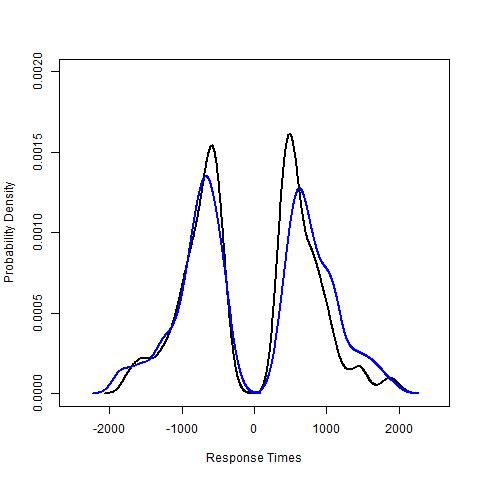
\includegraphics[width=0.9\textwidth]{Cond_distr_RRdata}
\caption{Correct and Error Probability Densities of Response Times}
\label{fig:conddist}
\end{figure}
%

A more complete understanding of relation between correct and error response times arises from examining performance on a multifactorial experiment like the benchmark data examined here.
One effective graphical summary of the whole experiment that can reveal the relation between correct and error response times is called a quantile-probability graph (QPG). QPG is a union of several quantile-probability functions that map proportions of correct or error responses into a response time quantile. Constructing a QPG requires to only pick the number and magnitude of quantiles. The \{0.1, 0.3, 0.5, 0.7, 0.9\} quantile set captures shapes of both correct and error response time density well, so I will use it to form a QPG  \citep{RatTue2002,RatMck2008}.

Figure \ref{fig:qp} shows a plot of a QPG for one subject presented with stimuli of different brightness either under speed or accuracy instructions. The error rates are represented on the abcissa below 0.5 and correct rates above 0.5. Each probability responds to a brightness ratio with easier ratio resulting in higher accuracy. The ordinate represents the response time quantiles stated above. Overall, five quantile-probability functions are displayed and their points are connected for clarity.

With a QPG one examine the relation between correct and error responses in more detail. If the QPG is approximately symmetric with respect to a vertical line passing through the point of chance performance, then correct and error probability densities do not differ. Asymmetry indicates differences between correct and error response times. The benchmark data results in an assymetric QPG in Figure \ref{fig:qp}. 
The pattern of differences between correct and error densities depends on the overall accuracy, itself manipulated by brightness level. When accuracy is high, the errors tend to be faster than correct responses. For moderate to lower accuracy, the errors tend to be slower than correct responses. The benchmark data shows what is called a cross-over pattern because other paradigms can show asymmetries where the errors are faster or slower under all conditions
\citep{RatTue2002,RatMck2008,Wag2009}.

Another pattern that stands out is the speed-accuracy trade off obtained by manipulating instructions \citep{Hei2014}. Instructing a subject to emphasize accuracy instead of speed results in shifting and rescaling both correct and error densities towards slower response times. The effect manifests itself in the upward movement and outward stretching of the QPG. At the same time, emphasizing accuracy improves accuracy for the same level of brightness. When accuracy improves, the QPG moves rightward and stretches outward.

Concentrating on either the speed or accuracy condition, the relation between response times and accuracy is different. Figure \ref{fig:qp} shows that the higher accuracy the faster the subject responds. This trend is present under both speed and accuracy instructions, and for both correct and error responses.

\begin{figure}
\centering
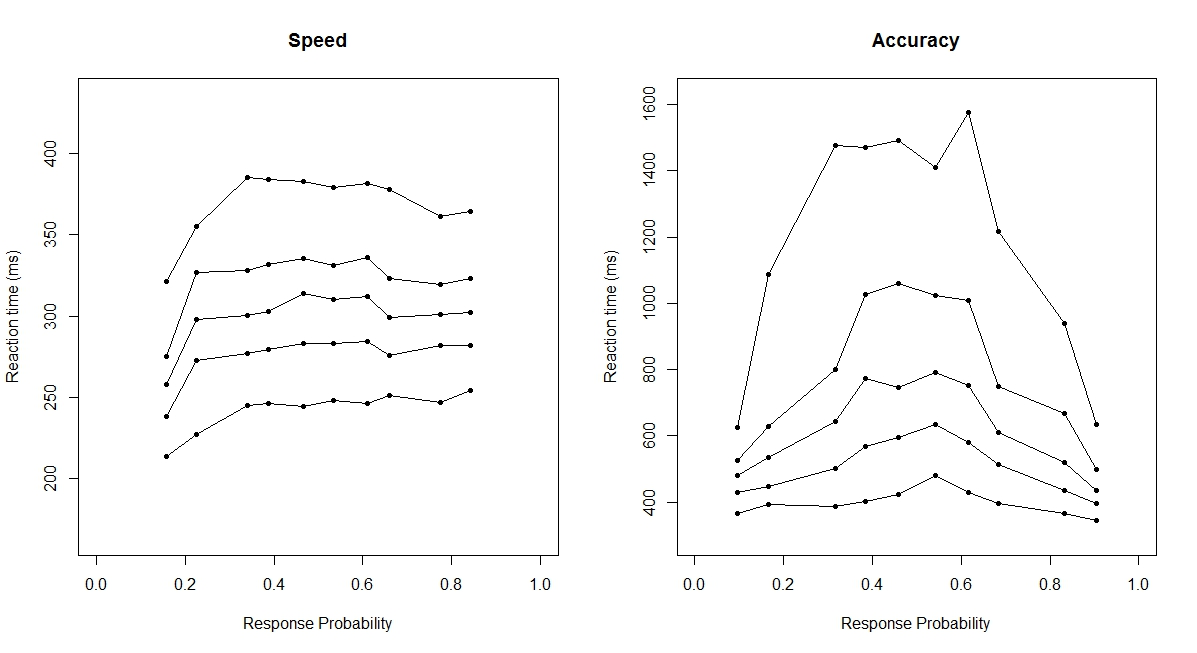
\includegraphics[width=0.9\textwidth]{QP_RRdata}
\caption{Quantile-Probability Graph}
\label{fig:qp}
\end{figure}
%

The last two aspects of the performance data are shown in Figure \ref{fig:autoacf} based on response times collected in two consequtive blocks. The first feature is presence of extreme response times. For example, the Trial Series plot shows that response nine took 538 ms, and response 21 lasted 196 ms. Relative to the rest of the responses these have extreme times. Other blocks show even larger deviations from the average.

The second feature is portrayed in the Auto-correlation plot. The dotted blue line represents a critical value for an alpha-level of 0.05 hypothesis test of zero auto-correlation. The benchmark data contains evidence for auto-correlation between response times stretching 6 trials. 
%
\begin{figure}
\centering
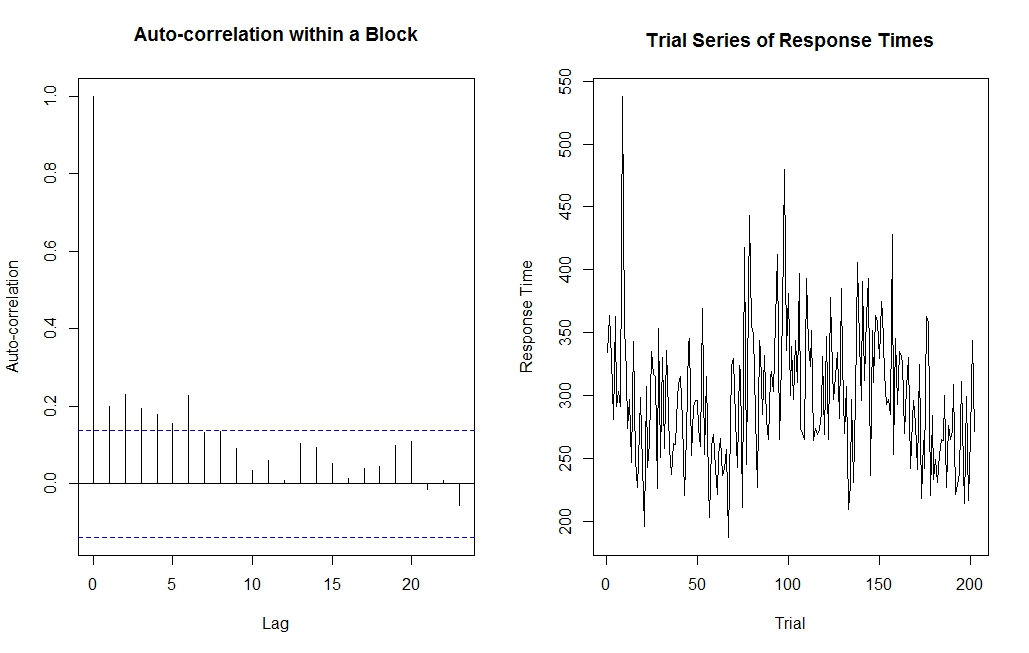
\includegraphics[width=0.9\textwidth]{Auto_Acf_RRdata}
\caption{Autocorrelation Function and Trial Series}
\label{fig:autoacf}
\end{figure}
%

The complete pattern of data features including speed-accuracy tradeoff, amount of variation in response times, skew of the conditional densities, relation between correct and error response times, relation between response time and accuracy, extreme response times and auto-correlation in response times provide strong constraints for developing and testing models of decisions. I will use features found in the benchmark dataset to discuss models of decision making and test proposed generalizations.

%%%%%%%%%%%%%%%%%%%%%%%%%%%%%%%%%%%%%%%%%%%%%%%%%%%%%%%%%%%%%%%%%%%%
\subsection{Sequential Sampling Models}

A common approach to modeling cognitive processing underlying two-choice
tasks is to decompose them into processes of encoding of stimulus features, response selection based on a relevant stimulus feature and motor execution. A cognitive process model for these tasks should make sufficient assumptions about these processes to predict patterns in performance
data. A delicate balance has to be struck between what processing details to include
and what details to exclude from models  because it will determine their generalizability across two-choice tasks. For instance, including details about how lexical information is accessed in
memory to direct response selection will make a model inapplicable to
brightness discrimination. The dominant approach to this balancing problem
is sequential sampling models.
    
A fundamental theoretical assumption of sequential sampling models
is that the same general decision process operates across all two-choice
tasks. Then, a generalizable model should provide a detailed account of the
decision process while making few assumptions about the stimulus encoding
and motor processing. Over the last $~50$ years, many models of this type
have been developed, and some of the most successful ones
can explain all the major patterns in the response time and response data,
under a variety of experimental conditions and tasks
\citep{Sto1960,Rat1978,RatTue2002,Smi1995,UshMcc2001,BroHea2008}. Some
models have also been used for predicting firing rates in neural
populations representing choices
\citep{RatChe2003,RatHas2011,SmiRat2004,Bog2007}, but I will concentrate on
performance data.
    
The underlying principle of sequential sampling models is that when an
observer is tasked with selecting the correct response, in limited time
from a noisy stimulus, he or she samples and accumulates
information from the relevant stimulus attribute until one of two
decision thresholds is reached
\citep{Sto1960,Edw1965,Pik1973,Rat1978,UshMcc2001,RatSmi2004,SmiRat2004,
RatMck2008,Wag2009,Luc1986,TowAsh1983,BogBro2006}. By controlling
these thresholds, the observer can balance the trade-off between
speed and accuracy of responses \citep{BogWag2010}. Thresholded accumulation of information naturally provides
predictions of performance data collected during two-choice
tasks. For example, accumulation times vary from run to run to produce distributions of
response times and which threshold is reached first determines the
response.
    
Given the sequential sampling principle, any concrete model of simple
decisions makes detailed assumptions about the nature of sampled
information, temporal structure of sampling, stopping rule and sources of
randomness \citep{RatSmi2004,BogBro2006,TeoUsh2013}. Combinations of
modeling assumptions generate the range of possible sequential sampling
models. For example, the sampled information can consist of discrete or
continuous packets. The size of the packets may be fixed or variable. The
accumulation of information packets may happen at fixed or variable
discrete time points, or continuously. The stopping rule may be absolute,
in which case accumulation stops when evidence in favor of one of the
choices reaches a threshold, regardless of the amount of evidence favoring
the alternative. In contrast, the relative rule requires that evidence
favoring one of the choices has to exceed the other by some amount.
    
Examples of sequential sampling models include a random walk model that
stops accumulation of discrete packets of randomly varying information over
discrete time according to a relative rule \citep{Lam1968}, a Poisson
counter model that continuously accumulates discrete, fixed information
packets until evidence for either of the choices reaches a threshold
\citep{Lab1962}, and a Wiener diffusion model that describes accumulation
of continuous packets in continuous time until a relative threshold
\citep{Rat1978}. I will concentrate on an empirically successful Ratcliff
diffusion model \citep{RatTue2002} as a base for incorporating assumptions
about process associations.
    
%%%%%%%%%%%%%%%%%%%%%%%%%%%%%%%%%%%%%%%%%%%%%%%%%%%%%%%%%%%%%%%%%
\subsection{Ratcliff Diffusion Model}

The Ratcliff diffusion model is a variant of the Wiener diffusion model
\citep{Lam1968,LinHea1975,Rat1978,RatRou1998,RatTue2002}. I
concentrate on this model because of its long development \citep{Rat1978,RatRou1998,Rat2002,RatTue2002,Rat2013}, and successful
testing against a wide range of experimental data \citep{RatMck2008,Wag2009}. In the following subsection I present a mathematical description of the Ratcliff model,its psychological interpretation, and show what features of performance data the model can and cannot predict.
    
Underlying the Ratcliff model is a drift-diffusion Wiener process, a special case of a continuous time, continuous state space
diffusion process that begins at some starting point and evolves until
it reaches one of two absorbing boundaries\citep{Ros2014,KarTay1975,KarTay1981}. Formally, a Wiener process is an
uncountable, ordered collection of univariate random variables 
%
\begin{equation} 
\{X(t); t \in T\} 
\end{equation} 
% 
with the index set $T \in [0, \infty)$ \citep{KarTay1981,Smi2000}. Given two absorbing boundaries at $0$ and $\alpha>0$, and a starting point
$\zeta \in (0, \alpha)$, the state space $S$ of $X(t)$ is the
interval $[0, \alpha]$. A realization of the Wiener process $X(t) = x(t)$, called a sample path, is a real-valued univariate function that maps index set into state space. $x(t)$ describes a particular sequence of states through which the Wiener process evolves.

Evolution of the drift-diffusion Wiener process is characterized by drift and diffusion coefficients. A drift coefficient, $\delta = \lim_{\Delta t \to 0}\frac{1}{\Delta t}\mathrm{E}\left[X(t + \Delta t) - X(t) \mid X(t) = x\right] \in \mathbb{R}$, quantifies mean instanteneous change in the state of the process and a diffusion coefficient, $\sigma^2 = \lim_{\Delta t \to 0}\frac{1}{\Delta t}\mathrm{Var}\left[X(t + \Delta t) - X(t) \mid X(t) = x\right] > 0$, quantifies mean instantaneous squared change in the state of the process. 

The drift coefficient determines the direction and magnitude with which an instance of the Wiener process tends to evolve towards a boundary. Positive values bias evolution towards $\alpha$ and negative values towards 0, while the value of $\delta$ controls how rapidly the process approaches an absorbing boundary. In contrast, the diffusion coefficient determines variability in evolution. For small values the state of the process may fluctuate a bit, but for large values the process may show large fluctuations in direction and moment-to-moment transitions.

There are several ways to
complete definition of the Wiener process assuming the above facts. One way is to describe properties
of an arbitrary point, $X(t)$, and increments, $X(t_2) - X(t_1)$, of the process. The drift-diffusion Wiener process with absorbing boundaries 
satisfies
%
\begin{enumerate} 
\item $X(t)$ is an almost surely continuous function,
%
\item $X(0) = \zeta,$ where $0 \le \zeta \le \alpha$,
%
\item $X(t) \sim \mathcal{N}(\delta t, \sigma^2 t)$,
%
\item increments are stationary, that is for $t_1, t_2 \in T$, where $0 < t_1 < t_2$, $X(t_2) - X(t_1)$ is equal in distribution to $X(t_2 - t_1)$, and
%
\item if for $t_1, t_2, \ldots, t_n \in T$, with $t_1 < t_2 < ... < t_n$, the increments $X(t_1),
X(t_2) - X(t_1), \ldots, X(t_n) - X(t_{n-1})$ are independent.
\end{enumerate} 
%


Another definition arises from considering the evolution of the Wiener process,
formalized by the linear, first-order stochastic  differential equation 
% 
\begin{equation}
\label{eqn:sde}
dX(t) = \delta dt + \sigma dW(t) 
\end{equation} 
% 
where $\delta$ and $\sigma$ are defined as above, $W(t)$ is a
standard Wiener process with points distributed as normal
variates with mean 0 and variance $t$. The Wiener process $X(t)$ is a unique solution to the Equation \ref{eqn:sde}.

In addition to its mathematical assumptions, the Ratcliff
diffusion model provides linking assumptions that
map the process and its parameters into a psychological process and variables relevant to describing a decision mechanism. In line with sequential sampling approach to decision making, the drift-diffusion Wiener process models a perfect, but noisy integrator of relative information. Integrator starts at some initial amount of decision-relevant information and continuously accumulates continuous information samples without loss \citep{Smi2000,BogBro2006}. 

The index set $T$ describes the time passed from beginning of accumulation, and the state space $S$ describes the possible amounts of information that an integrator can hold under certain conditions.  The drift coefficient $\delta$ is interpreted  to measure the average rate of information uptake by a perfect integrator, and the
diffusion coefficient $\sigma^2$ describes the level of noise in
the information uptake. 

Boundaries of
the state space, 0 and $\alpha$, represent decision thresholds that quantify the amount of relative information
needed to form a decision. The lower and upper bounds
could represent one of two
choices, say ``No'' and ``Yes'' in the auditory signal detection
experiment.  The separation between boundaries, $\alpha$, quantifies decision
caution, with larger separation implying that more
information is required before making a decision.
    
The starting point $\zeta$ of the process represents the initial
amount of information from which the accumulation process
begins. The level of initial information represents the bias an
observer may have towards one of the choices. The farther away from $\alpha / 2$ the starting point $\zeta$ is, the more initial information there is for a particular choice. The initial information asymmetry suggests an alternative parameterization of the Wiener process corresponding to a biased integrator that starts accumulation with bias $\beta = \zeta / \alpha \in [0, 1]$, a proportion of the distance from 0 to $\alpha$.
    
The drift-diffusion Wiener process model of a perfect integrator provides a natural way to
predict the joint probability density of decisions and decision times in a two-choice task. A sample path of the drift-diffusion
Wiener process will start at $\zeta$ (or $\beta$) and take some random time to
absorb at one of the boundaries. Let $T^d > 0$ be the time to absorption and $R \in \{0,1\}$ be the randomly passed boundary at $T^d$. Translating into psychological terms, the sample path is evolution of the information integrator to a decision $R$ during the duration of decision time $T^d$. The model predicts that the probability of
decision $R = 1$ is
%
\begin{equation}
\label{eqn:prob}
P(R = 1) = \left[\exp\left(\frac{-2\delta \zeta}{\sigma^2}\right)-1\right]/
                \left[\exp\left(\frac{-2\delta \alpha}{\sigma^2}\right)-1\right].
\end{equation}
%

In addition to probabilities of decision, the model predicts joint variation of decisions and decision times. The upper bound component of the joint probability density function of $T^d$ and $R$ is
%
\begin{eqnarray}
\label{eqn:wd}
\lefteqn{f(t^d, 1 \mid \alpha, \delta, \zeta, \sigma^2) =} \nonumber \\
& & \frac{\pi\sigma^2}{\alpha^2}\exp\left(\frac{\delta\zeta}{\sigma^2}-\frac{\delta^2t^d}{2\sigma^2}\right)
\sum_{k=1}^\infty{k\exp\left(\frac{-k^2\pi^2\sigma^2t^d}{2\alpha^2}\right)
\sin\left(\frac{k\pi(\alpha - \zeta)}{\alpha}\right)},
\end{eqnarray}
%
and the lower bound component is obtained by replacing $\delta$ with 
$-\delta$ and $\alpha - \zeta$ with $\zeta$.  

The form of the Equation \ref{eqn:wd}
suggests that distributional prediction of the Wiener process model suffers from lack of identifiability %\citep{DonBro2009}. 
A model is identifiable when for any, nonequivalent parameters $\theta_1, \theta_2 \in \Theta$, the resulting probability density functions are unique, that is $f(x \mid \theta_1) \neq f(x \mid \theta_2)$ \citep{CasBer2002}. As a result, identifiability of a  model creates a possibility of precise estimation of true parameters with an infinite sample size. For Equation \ref{eqn:wd},
assuming that $\{\alpha,\delta,\zeta,\sigma^2\}$ are free to vary, if one multiplies all parameters of the model by a factor $c$, then the predictions do not change. Thus, parameter recovery is unique upto a scaling operation. 

For the Wiener model, resolving lack of identifiability requires fixing one of the parameters to an arbitrary value. Typically, application of the Wiener model relied on fixing the diffusion coefficient $\sigma^2$ to 0.1 or 1 \citep{Rat1978,RatTue2002,RatMck2008}.The psychological interpretation of fixing $\sigma^2$ is that the noisiness of the integrator is the same across conditions, and that experimental manipulations have to be explained in terms of the remaining parameters. The stability of noise is a theoretical assumption, and ultimately should be tested against a particular experimental situation. Given that this thesis concentrates on the \citet{RatRou1998} data, which was generated without manipulations aimed at changing noisiness of the integrator, I will assume that $\sigma^2 = 1$, across all experimental conditions, to resolve identifiability issue.
 
The model specified so far allows predictions only about $T^d$, which represents the unobservable 
decision time. To fully connect the Wiener process to performance
data, the model requires assumptions about the perceptual and motor
processes surrounding the decision stage. A  sufficient adjustment is to relate the decision time to respone time because the response is coupled to the decision in two-choice tasks.

An additive decomposition of two-choice tasks implies that
before information sampling can begin, the sensory stimulus has to be
transduced and its features encoded. When the accumulation reaches one
of the thresholds, the observer has to organize and execute a motor
response for their decision to become observable. The mechanistic details of such
perceptual and motor processing are typically not specified when specifying a sequential sampling model (but see
\citet{SmiRat2009}), but their time can be captured by a single parameter
$\tau^er$. Then, response time
%
\begin{equation}
T^{rt} = T^d + \tau^{er}
\end{equation}
%
where $T^d$ is the decision time and $\tau^{er}$ is the combined perceptual
and motor processing (non-decision) time. If $\tau^{er}$ is a
constant, the joint probability density of response times and responses is
a shifted density of decision times and decisions
%
\begin{equation}
f(t^{rt} - \tau^{er}, r \mid \alpha, \delta, \zeta, \sigma^2) = f(t^{rt}, r \mid \alpha, \delta, \zeta, \sigma^2, \tau^{er}).
\end{equation}

Comparison of the Wiener model's predictions with experimental data shows that, for some experimental paradigms, the model can accurately predict several qualitative and quantivative features of performance data. First, the large variation in response times, as shown in Figure \ref{fig:conddist}, arises from within-trial variability in accumulation. Variability follows because sometimes the integrator uptakes information rapidly resulting in a fast response time. On other trials, the integrator may oscillate for a while around the middle or one of the bounds before terminating, leading to a slow response time. 

Second, noisy within-trial accumulation accounts for errors. To model accuracy one has to assume that the starting point $\zeta = \alpha /2$, the drift rate $\delta \geq 0$ and boundaries represent correct (upper) and error (lower) responses. The starting point restriction reflects an assumption that there is no bias towards correct or error responses, and the non-negative drift rate represents the assumption that stimulus information  restricts performance to be between chance and full accuracy. With these assumptions,  noisy accumulation sometimes results in the integrator terminating at the lower bound, which causes an error. 

Third, the decision model based on the Wiener process can predict the positive skew of response time densities observed in Figure \ref{fig:conddist}. The Wiener process tends to move directly towards one of the bounds, and only sometimes oscillates between the bounds or reverses its course, which predicts that A and B response time probability densities (or correct and error) will have a positively skewed shape.

Fourth, the model can explain the speed-accuracy trade off. Experimentally, the speed-accuracy is obtained by manipulating performance instructions. The Wiener model predicts the trade off, like the one in Figure \ref{fig:qp}, by adjusting the threshold parameter, $\alpha$, or, in psychological terms, instructions manipulate subject's caution level. Assuming an equidistant starting point, $\zeta = \alpha /2$, and $\alpha$ representing the correct response, then increasing $\alpha$ will result in the integrator taking a longer time to produce the correct response. The farther distance from $\zeta$ to 0 will also increase accuracy by allowing some of the accumulationg paths initially moving towards the error bound to reverse their trajectory towards the correct bound.

Fifth, the Wiener model predicts that with higher accuracy subject's correct response times will tend to be faster. 
This pattern is observed for both  speed and accuracy instructions, as shown in Figure \ref{fig:qp}. When instructions are fixed, only the stimulus quality is manipulated. Intuitively, with better stimulus information the task becomes easier, so the accuracy goes up and processing time is faster.The observed relation is predicted by assuming that the quality of stimulus, such as the ratio of white to black pixels, modulates the drift rate. When boundaries represent correct and error responses, the Wiener model captures the joint effect because increasing the drift rate forces accumulation to move more rapidly and more frequently towards the correct bound. 

The five features captured by the Wiener model is only a fraction of the full collection of regularities found in the benchmark and other datasets. The model is theoretically inadequate to account for asymmetric relations between correct and error response times, additional variation in the left tail of the response time density, auto-correlation or extreme observations. 
    
Motivated by some failures of the Wiener model, the Ratcliff model adds additional structure to the Wiener process that helps to account for asymmetry between correct and error response times as well as additional left tail variation. The solution to these empirical failures is to
propose additional noise in cognitive processing, which
manifests itself in random fluctuations of processes across
trials. Specifically, the Ratcliff model assumes that there is trial-to-trial variation in stimulus quality, stimulus encoding, initial state of the integrator and motor execution varies in time. 

Mathematically, the idea of processing variation can be modeled with the drift-diffusion Wiener process with
parameters varying across trials according to some distribution. Thus, and that a
sample of response times is due to a mixture of Wiener processes evolving under different combinations of parameters.
The full Ratcliff diffusion model
assumes that the starting point $\zeta$, non-decision time $\tau^{er}$ and drift rate $\delta$
are random variables with probability densities
%
\begin{eqnarray}
\zeta & \sim & \mathcal{U}(\lambda - \frac{\gamma}{2}, 
\lambda + \frac{\gamma}{2}), \nonumber \\
\tau^{er} & \sim & \mathcal{U}(\chi - \frac{\phi}{2}, 
\chi + \frac{\phi}{2}), \text{and} \nonumber \\
\delta & \sim & \mathcal{N}(\nu, \eta),
\end{eqnarray}
%
where $\lambda > 0$ and $\chi > 0$ are mean parameters, $\gamma > 0$ and $\phi >0$ are range parameters, $\nu \in \mathbb{R}$ is a mean parameter and $\eta > 0$ is a standard deviation parameter. To make sure that the starting point is within the state space and nondecision is positive, the parameters satify $0 < \lambda - \frac{\gamma}{2} < \lambda + \frac{\gamma}{2} < \alpha$) and $0 < \chi - \frac{\phi}{2}$), respectively.

The distributional assumptions for
$\zeta$, $\tau_{er}$ and $\delta$ were made for numerical
simplicity \citep{Rat1978,RatRou1998,RatTue2002}, and have become traditional
assumptions for estimation methods that find best-fit parameters by optimizing a measure of goodness-of-fit \citep{Tue2004,VanTue2007,VosVos2007}. A natural concern is sensitivity of model predictions and substantive conclusions to assumptions of across-trial variability.
\citep{Rat2013} demonstrated that the model fit is robust with
respect to a wider class of distributions. For a wide range of parameters, swapping beta for normal distribution of drift, beta for uniform starting point, normal or exponential for uniform nondecision time, one at a time, resulted in accurate recovery of parameters and the same substantive conclusions. Except for extreme parameter values, assumption of exponentially distributed nondecision time, or normally distributed nondecision time with small boundary $\alpha$, the study showed that empirical success of the model is moderately insensitive to across-trial variability assumptions. 

The Ratcliff assumptions imply that the first passage density is a
statistical mixture model with joint density function
%
\begin{eqnarray}
\label{eqn:mixture}
\lefteqn{f(t^{rt}, r \mid \alpha, \lambda, \gamma, \nu, \eta, \chi, \phi) =} \\ 
& & \iiint\limits_V f(t^{rt}, r \mid \alpha, \zeta, \delta, \tau^{er})f(\zeta \mid \lambda, \gamma)f(\delta \mid \nu, \eta)f(\tau^{er} \mid \chi, \phi)d\zeta d\delta d\tau^{er} \nonumber,
\end{eqnarray}
%
where $r=0,1$ and the individual densities have been specified above.

This probability density determines all the falsifiable predictions
of the Ratcliff diffusion model for two-choice performance data and can
accurately describe the five features of performance data mentioned above as well as account for two additional features\citep{RatTue2002, Rat2002}. 

The first additional data feature the Ratcliff model can handle is occasional assymetry between correct and error mean response times \citep{RatMck2008, Wag2009}. There are three basic patterns that can arise: slower errors, faster errors, and a cross-over pattern where under high accuracy errors are faster and under low accuracy errors are slower. The benchmark data shows a cross-over pattern, as shown in Figure \ref{fig:qp}. These patterns are very diagnostic, and have been a long target for model development \citep{Lam1968,Rat1978,RatRou1998}.

The Ratcliff model can handle all three asymmetry patterns using the across-trial variation assumptions. The slow errors arise only from assuming that the drift rate $\delta$ follows a normal distribution. Psychologically, the variable drift represents the noisy nature of the representational process that provides a somewhat different neural activation pattern when presented with exactly the same stimulus pattern. How drift variation produces slow errors can be understood by considering that the mean correct and error response times for the mixture model are weighted averages of correct and error means conditioned on a drift rate value. 

Assume that $T_c^{rt}$ is the correct response time and $T_e^{rt}$ is the error response time. Then, assuming only the drift rate varies, the correct mean of the mixture model
\begin{equation}
\mathrm{E}\left[T_c^{rt}\right] = \mathrm{E}_\delta\left[\mathrm{E}\left[T_c^{rt} \mid \delta\right]\right] = \int_\mathbb{R}\mathrm{E}\left[T_c^{rt} \mid \delta\right] f(\delta)d\delta,
\end{equation}
and similarly the error mean of the mixture model
\begin{equation}
\mathrm{E}\left[T_e^{rt}\right] = \mathrm{E}_\delta\left[\mathrm{E}\left[T_e^{rt} \mid \delta\right]\right] = \int_\mathbb{R}\mathrm{E}\left[T_e^{rt} \mid \delta\right] f(\delta)d\delta,
\end{equation}
where $f(\delta)$ is a normal density with mean $\nu$ and standard devation $\eta$. In a usual experiment $\nu$ is positive, so the mass of the $f(\delta)$ is heavily distributed over positive numbers. For a positive drift rate, the error mean is slower than the correct mean.  Thus, averaging mean correct and error response times with respect to $f(\delta)$ will result in upweighing fast correct means and slow error means. Hence, the overall mixture pattern would be slower errors.

Fast errors can be incorporated into a sequential sampling model by assuming variability in the starting point $\zeta$. With drift rate fixed to a positive value, most Wiener processes will tend to terminate at the correct bound, so for errors to occur the process has to rapidly evolve towards the lower bound. Thus, mean error response times for different starting values will tend to be faster than mean correct response times for symmetric starting values. When equilly weighted by the uniform density, the mixed means will result in faster errors.

Combination of variability in the drift rate and starting point in the Ratcliff model can produce all three patterns. The switch between different patterns lies in relative variability of the drift rate and starting point. When variability of the drift rate is sufficiently higher than variability of the starting point, the slow errors pattern arises. Reversing the relation will result in fast errors. The model predicts a cross-over, with fast errors at low accuracy and slow errors at high accuracy, when variability is similar for the two parameters.

The second additional pattern the Ratcliff model predicts is extra variabiliy in the lower tail not predicted by the wiener model. Figure \ref{fig:qp} shows the level of lower tail variability as measured by the 0.1 quantile. Assuming trial-to-trial variability in the nondecision $\tau^{er}$ allows the Ratcliff model to predict this empirical pattern. The reason is that the nondecision parameter sets the lower bound on the fastest response time, so the effect of across-trial variation is strongest in the left tail. 

Even with all the variability assumptions, the Ratcliff model still cannot capture two important
features of performance data. First, it is typical to observe extremely fast or slow response times within a series of trials, and second, serial dependencies among responses and response time are ubiquitous, as evidenced in the Figure \ref{fig:autoacf} for the benchmark data. Several studies have proposed how to model these features \citep{RatTue2002,VanTue2007,GaoWon2009,CraPer2010,JonCur2013}. The auto-correlation in the response times can be captured by assuming that next trial parameters somehow depend on the current or even past trial parameters. Learning and information carry-over are two plausible psychological process that could underlie such auto-correlation.
In constrast, the extreme response times can be accounted by fast guesses or delayed decisions, and modeled with a mixture of Wiener processes, delayed Wiener processes and guess process. However, auto-correlation and extreme values do not seem to be important data features to account for if trying to understand cross-correlation between parameters.

Preliminary investigations of the effects of correlated parameters on performance data show no effect on auto-correlation or increase in proportion of extreme values. Only a model that can accurately capture conditional response time distributions and various relations between correct and error response times, or response time and accuracy, is required to study cross-correlation between parameters. The Ratcliff model does a superb job of fitting features affected by cross-correlation, therefore I will use it as a base for generalization.
    
The standard Ratcliff model has no principled mechanisms to explain dependence between parameters over trials.
In other words, parameters that vary across-trials are assumed to be statistically independent. Therefore, the model cannot be used to make inferences about the coordination among processes
across trials. This limitation leads me to propose a generalized
Ratcliff model that can be modified to accommodate different covariance
structures across parameters.

%%%%%%%%%%%%%%%%%%%%%%%%%%%%%%%%%%%%%%%%%%%%%%%%%%%%%%%%%%%%%%%
\section{Problems to be solved}

In this section I will elaborate on problems addressed by this thesis. The first part discusses incorporation of parameter covariance into the diffusion model, and the second part discusses exploration and testing of modified models.

\subsection{Diffusion model with covarying parameters}

\trish{Notes on below: As above, simply saying that we've never tested the
independence assumption before is not a good motivation for what you're
proposing.  The Ratcliff model fits unbelievably well without it, and further
improvements in fit are not likely to be worth the effort to develop any
generalizations of the model.  You need to motivate this from data and theory.  This
needs to be done above, not here.  Here you can simply reference your
earlier arguments.}

The goal of this proposal is to develop a generalization of
the Ratcliff diffusion model that can help to make inferences about
coordination of cognitive processes across trials. The Ratcliff model
assumes mutual independence of noisy parameters. However, this
assumption has not been directly tested. Testing the assumption
will require specifying a multivariate density for the process
parameters that permits estimating the dependencies among them.
Fits of this generalized model can then be compared statistically
to the fits of the independent model to performance data.
    
There is a stock of common multivariate densities that could be used
to model dependence, including the normal, t, gamma, and F
\citep{KotBal2004}. However, these densities are too restricted to
be of use. Without
reparameterization, the parameters of the Wiener first passage do not have
infinite supports, and the supports are not independent.  The starting
point $\zeta$, for example, is constrained to be between 0 and the
threshold parameter $\alpha$.
In addition, the common distributions all have the same univariate
marginal densities, whereas it will be more useful to assign
different functional forms to different parameters
\citep{Rat2013}. These considerations suggest that new multivariate
densities need to be constructed to generalize the Ratcliff model.

The problem of constructing a
new multivariate density can be broken down into three sub-problems:
\begin{enumerate}
\item picking a parameterization of the Wiener process,
\item picking a dependence structure among the three parameters, and
\item picking marginal probability densities for each parameter.
\end{enumerate}

\trish{Note: Why aren't you using this structure (sub-problems) for the
subsections below?  And then in the first subsection below, you list three
more problems.  This is very distracting.}

%%%%%%%%%%%%%%%%%%%%%%%%%%%%%%%%%%%%%%%%%%%%%%%%%%%%%%%%%%%%%%%%
\subsection{Properties of models with dependencies}					     


\trish{Note: I assume below that you are talking about the relative
contributions to goodness of fit of the different parts of the model.  You
need to state that explicitly.  If it is something else, you need to say
that explicitly.  Rewrite this:}

Developing the proposed
generalization gives rise to three  problems. The
first problem is to understand the effects of the association structure
of the parameters on predictions of response time and response
proportion. Given the complexity of the model it is not clear a priori
whether association structure will result in noticeable effects on performance data. It is possible that the first passage density component and
univariate marginals of variable parameters will overpower the association
structure implying little change in behavioral predictions from the Ratcliff model. If it
is negligible, then models with really different association structures
will mimic each other. The mimicry will undermine the precision of the
proposed models to infer presence and character of process coordination
across trials. The crucial comparison is relate proposed models to the
independent model.
    
If association structures are \trish{explain, see above: discriminable via
performance data}, then studying predictive properties of proposed models
will provide information about the empirical signature of process
coordination and will reveal experimental conditions under which
associations create detectable changes in performance.  Obtaining
performance predictions requires evaluating a mixture model of response
times and responses. The mathematical form of the mixture model arises from
combining the Wiener first passage density and a new multivariate model of
across-trial parameter variation through integration. The required
integration is not tractable \citep{Tue2004}. Thus, the problem of
obtaining predictions is primarily to find an algorithm to approximately
evaluate a mixture density.
    
The second problem is to understand estimation
properties of the proposed models. Before applying models to performance
data it is important to ensure that their parameters can be accurately
estimated from sample sizes found in experimental literature. Without an
accurate estimator fitting the model to real data is pointless because
inferences will be unreliable. Fitting diffusion models has become a topic
of its own in psychology with several approaches to choose from
\citep{VosVos2007,RatTue2002,VanTue2007,VanTue2011}. Some of these
procedures have been developed strictly for the Ratcliff diffusion model
while others can be extended flexibly to incorporate a diffusion model with
an association structure. Hence, the second problem is to find an
estimation procedure that can fit a complex mixture model accurately and in
reasonable time.
    
Lastly, the proposed models have to be fit and evaluated against real
data. The purpose of generalizing diffusion models is to
obtain novel insights from data. Given a set of competing models,
including some that have an association structure and a model
that does not, there needs to be a clear evaluation criterion
to select among them. None of the models inherently suffer from lack
of substantive interpretation or plausibility, so evaluation has to
proceed on how well the models account for data adjusted for
complexity \citep{CavMyu2013}. Addition of an association structure
comes at a cost of three parameters and increased functional
complexity, and to be taken seriously it needs to fit the data
substantially better than the independent model. 

\trish{Note: I think
you should focus on fitting new data, not fitting old data better.}


Thus, the last problem is to pick quantitative and/or graphical methods to evaluate fit while adequately adjusting for
complexity of the proposed models.


%%%%%%%%%%%%%%%%%%%%%%%%%%%%%%%%%%%%%%%%%%%%%%%%%%%%%%%%%%%%%%%%
\section{Proposed Methodology}

In this section I will provide details of how I will address the posed problems. First, I will present theory of copulas and show how one can use them to construct mixing model of dependent variables. Second, I will describe a Monte Carlo method to obtain performance predictions for the proposed models. Lastly, I will present Bayesian methods of statistical inference, including hierarchical models, Markov Chain Monte Carlo sampler and posterior sample diagnostics, model selection, posterior predictive checks, broken up into several subsections.

\subsection{Copula-based modeling of associations}

Development of cognitive process models, that describe an association
structure between component processes involved in a sequence of simple
decisions, requires selecting a multivariate distribution
for the covarying parameters. In the context of modeling speeded decisions with the Ratcliff model, this
problem is both underconstrained, given the lack of information about
the association structure, and restricted, because the
parameters are scaled differently. Hence, the method of
construction should allow combining an arbitrary association
structure and arbitrary univariate marginals. 

The framework of copulas, developed in probability theory over the
last 60 years and recently imported for data analysis in a variety of
fields, is well-suited for this problem
\citep{Skl1959,Joe1997,Nel2007,BerWoo2008}. Mathematically, a copula is a function
$C(u_1, u_2, \dots, u_p): [0, 1]^p \mapsto [0, 1]$ that maps a
point $(u_1, u_2, \ldots, u_p)^T$ from a
$p$-dimensional unit hypercube to a point in a unit interval.
Probabilistically, a copula is a probability distribution on a standard
hypercube with continuous, uniformly distributed univariate marginals
$U_i \sim \mathcal{U}(0, 1), i = 1, 2, \dots, p$. Figure \ref{fig:copula} shows samples drawn from four copulas with approximately matched level of dependence including normal, Clayton, Gumbel and Frank. 

\begin{figure}
\centering
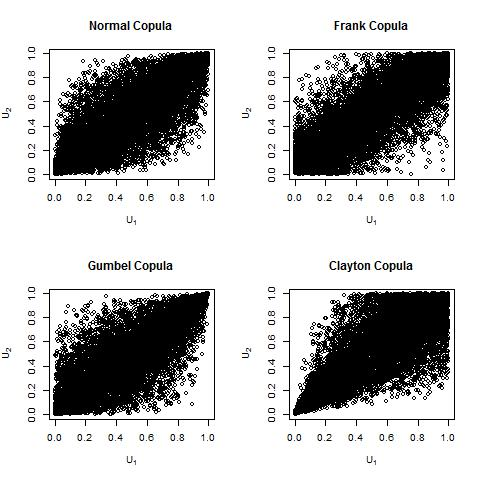
\includegraphics[width=0.9\textwidth]{4_Copulas}
\caption{}
\label{fig:copula}
\end{figure}

The fundamental result that makes copulas important for constructing models with dependent variables is due to Sklar's \citeyear{Skl1959} two-part representation theorem:
%
\newtheorem*{Sklar}{Theorem} 
\begin{Sklar} 
Let $F$ be a multivariate distribution with continuous marginal
distributions $F_1, F_2, \dots, F_p$, then there exists a unique
copula $C$ such that 
\begin{equation}
\label{eqn:sklar}
F(x_1, x_2, \dots, x_p) = C(F_1(x_1), F_2(x_2),
\dots, F_p(x_p)).
\end{equation}Conversely, given a copula $C$ and marginal
univariate distributions $F_1, F_2, \dots, F_p$, F is a
multivariate distribution.  
\end{Sklar}

The forward implication of Sklar's theorem means that every distribution
can be rewritten in terms of a copula and univariate marginals. This
suggests that copulas encode the dependency structure stripped from
all the univariate marginal information like scale and
location. For example, consider a bivariate distribution
\begin{equation}
\label{eqn:bipar}
F(x_1, x_2) = 1 - \left(1 + \frac{x_1}{\theta_1} \right)^{-\theta_2} -\left(1 + \frac{x_2}{\theta_1} \right)^{-\theta_2} +\left(1 + \frac{x_1 + x_2}{\theta_1} \right)^{-\theta_2},
\end{equation}
where $\theta_1 > 0$ is a scale parameter, $\theta_2 > 0$ is a shape parameter, and $x_1, x_2 \geq \theta_1$
\citep{FreVal1998}. The univariate marginal distribution for Equation \ref{eqn:bipar},
\begin{equation}
F_i(x_i) = 1 - \left(1 + \frac{x_i}{\theta_1}\right)^{-\theta_2}, i = 1, 2,
\end{equation}
is a Pareto distribution. Taking the univariate marginal form into account and rearranging the terms of Equation \ref{eqn:bipar} results in
\begin{eqnarray}
F(x_1, x_2) & = & F_1(x_1) + F_2(x_2) - 1 \\ \nonumber
& + & \left[(1 - F_1(x_1))^{-1/\theta_2} + (1 - F_2(x_2))^{-1/\theta_2} - 1 \right]^{-\theta_2}.
\end{eqnarray}
The bivariate distribution is a function of $F_1(x_1)$ and $F_2(x_2)$, so by Sklar's forward implication, its copula
\begin{equation}
\label{eqn:parcop}
C(u_1, u_2 \mid \theta_2) = u_1 + u_2 - 1 + [(1 - u_1)^{-1/\theta_2} + (1 - u_2)^{-1/\theta_2}]^{-\theta_2},
\end{equation}
where $u_1, u_2 \in [0, 1]$. Pareto marginals and the copula in Equation \ref{eqn:parcop} provide an alternative way for representing the bivariate distribution, where joint and marginal behavior of the variables is decoupled.

The converse implication of Sklar's theorem is a core result from the perspective of model building. It suggets that copulas and univariate marginals are basic building blocks that can be
combined in flexible ways to define new multivariate probability distributions. The copula method for constructing new models requires specifying an association structure of variables, represented by a copula, and individual features of the variables,  captured by univariate marginals. 

To demonstrate the usefulness of the converse implication consider construction of a bivariate distribution from exponential and Poisson univariate distributions, and a Clayton copula. A Clayton copula will impose a positive association with strong lower tail dependence. The exponential and Poisson distributions will make the variables positive, with one being continuous and the other discrete. Suppose the univariate $X_1$ is distributed exponentially with scale $\theta_1$, $X_2$ is distributed Poisson with scale $\theta_2$, and a Clayton copula has a probability distribution
\begin{equation}
C_C(u_1, u_2 \mid \rho) = \left(u_1^{-\rho} + u_2^{-\rho} - 1\right)^{-1/\rho},
\end{equation}
%\begin{equation}
%C_F(u_1, u_2 \mid \rho) = -\frac{1}{\rho} \log \left(1 + (e^{-\rho u_1}-1)(e^{-\rho u_2}-1) / (e^{-\rho}-1) \right),
%\end{equation}
where $u_1, u_2 \in [0, 1]$ and $\rho > 0$. Then, the converse part of Sklar's theorem implies, that a distribution of $X_1$ and $X_2$ is
\begin{eqnarray}
\label{eqn:newdist}
C_{Cl}(F_N(x_1), F_P(x_2) \mid \rho) = \\ \nonumber
\left(\left(1 - \exp(-x_1/\theta_1)\right)^{-\rho} + \left(\sum_{k = 0}^{\lfloor{x_2}\rfloor}\frac{\theta_2^k}{k!}e^{-\theta_2}\right)^{-\rho} - 1\right)^{-1/\rho}.
\end{eqnarray}
A sample from the new distribution is in Figure \ref{fig:newdist} with $\rho = 10, \theta_1 = 5$, and $\theta = 3$.
%
\begin{figure}
\centering
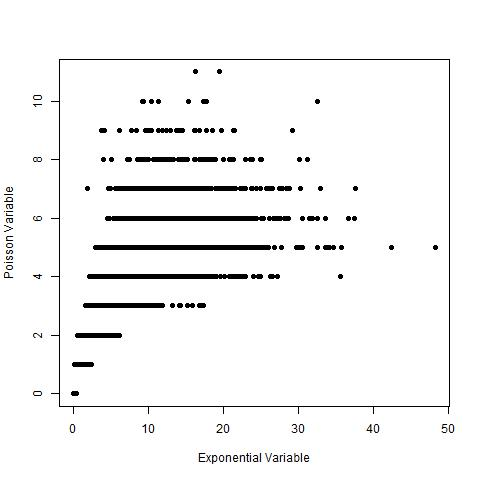
\includegraphics[width=0.9\textwidth]{Copula_model_ex}
\caption{}
\label{fig:newdist}
\end{figure}
% 
    
From  Sklar's theorem follow two useful
corollaries that shed more light on how copulas
are useful in constructing new multivariate distributions
\citep{Joe1997,Nel2007}. The first corollary is an alternative
representation of a multivariate probability density function:
%
\newtheorem{cors}{Corollary}
\begin{cors}
\label{thm:density}
For a differentiable p--dimensional distribution function with
continuous quantile functions $F_1^{-1},
F_2^{-1}, \dots, F_p^{-1}$, the probability density function
%
\begin{eqnarray}
f(x_1,x_2, \dots, x_p) & = &
\frac{\partial^p F(x_1, x_2, \dots, x_p)}{\partial x_1 \partial x_2 \cdots \partial x_p} \nonumber \\ 
 & = & \frac{\partial^p C(F_1(x_1), F_2(x_2), \dots, F_p(x_p))}{\partial x_1 \partial x_2 \cdots \partial x_p} \nonumber \\
 & = & c(u_1, u_2, \dots, u_p)\prod_{i = 1}^p f(x_i),
\end{eqnarray}
where $c(u_1, u_2, \dots, u_p)$ is the probability density of the copula, and $f(x_i)$ are probability densities of each dimension.
\end{cors}
%
The usefulness of
Corollary \ref{thm:density} is that it provides an alternative
way to construct a model by going directly to the probability density
function. This becomes useful when the distribution function has no analytical form. 

The results I have presented so far provide two routes for
defining new probability models (Sklar's theorem and Corollary \ref{thm:density}). However, any real application has
to be preceded by finding useful copulas \citep{Joe1997,Nel2007}. The
second corollary shows a simple way of obtaining a new copula:
%
\begin{cors}
\label{thm:copula}
Let $F$ be a p-dimensional distribution function with continuous
quantile functions $F_1^{-1}, F_2^{-1}, \dots, F_p^{-1}$, then for
every $(u_1, u_2, \dots u_p) \in [0, 1]^p$ a copula
%
\begin{equation}
\label{eqn:copula}
C(u_1, u_2, \dots u_p) = F(F_1^{-1}(u_1), F_2^{-1}(u_2), \dots, F_p^{-1}(u_p)).
\end{equation}
%
\end{cors}
%

Corollary \ref{thm:copula} implies that if one can specify an
existing multivariate distribution and derive its quantile functions,
then its copula is easily recoverable using
Equation \ref{eqn:copula}.  As a caveat, this method works
only if quantile functions can be obtained, which is not always
the case. 

Note that Sklar's theorem is another method for deriving copulas. The example involving the bivariate Pareto distribution led to derivation of its copula by knowing the joint distribution and clever rearrangement guided by knowledge of marginal distributions. This method is also limited because in many models rearrangements are often not obvious \citep{FreVal1998}. Fortunately, there are many other methods for finding new copulas, and the
literature provides a rich body of copulas to choose from to begin developing a model
\citep{Joe1997,Nel2007}.

Another useful consequence due to Sklar's result is that copulas provide a natural way for defining measures of dependence between random variables, regardless of univariate marginals. An often used scalar measure of linear dependence between random variables $X$ and $Y$ is Pearson's coefficient
\begin{equation}
\psi_P = \frac{\mathrm{Cov}\left[X, Y\right]}{\sqrt{\mathrm{Var}\left[X\right]\mathrm{Var}\left[Y\right]}},
\end{equation}
and it is natural samples coming from a normal or t distribution. However, Pearson's coefficient cannot be rewritten strictly in terms of a copula, and when the joint distribution is t, the coefficient may be undefined because moments may not be defined at low degrees of freedom. Another downside is that marginal distributions of X and Y have influence on the Pearson's measure through $\mathrm{Var}$ operator.

As an alternative, Kendall's  coefficient, which
measures the amount of monotonic dependence between two random variables,
can be defined strictly in terms of a bivariate copula \citep{Joe1997,Nel2007}.  For a bivariate random vector $(X, Y)^T$ drawn from a copula $C(\:)$ (with probability density $c(\:)$), the Kendall's coefficient equals
\begin{eqnarray}
\lefteqn{4 \iint_{[0,1]^2}C(u,v)c(u,v)dudv - 1} \nonumber \\ 
& = & 4 \mathrm{E}\left[C(U,V)\right] - 1.
\end{eqnarray}
Kendall's coefficent provides a convenient measure for comparing different copula-based models, and its estimate can provide a summary about relations of different parameters of the generalized Ratcliff model. Figure \ref{fig:copula} contains samples from four copulas with $\psi_K \approx 0.6$.

The tail dependence is a second scalar measure that can help to characterize dependence between random variables. This quantity considers dependence imposed by a copula only in the lower-left or upper-right quadrants. The tail dependence is defined as an asymptotic probability that the $X_2$ exceeds some quantile $q$ given that $X_1$ exceeds $q$. The  lower-left tail dependence
\begin{equation}
\lambda_L = \lim_{q \to 0}P\left(X_2 \leq F_2^{-1}(q) \mid X_1 \leq F_1^{-1}(q)\right), 
\end{equation}
and the upper-right tail dependence
\begin{equation}
\lambda_R = \lim_{q \to 1}P\left(X_2 > F_2^{-1}(q) \mid X_1 > F_1^{-1}(q)\right).
\end{equation}
Similar to the Kendall's coefficient, the tail dependence can be defined  strictly in terms of a copula $C(\:)$. For the lower-left tail, the dependence 
\begin{equation}
\lambda_L = \lim_{q \to 0^+}\frac{C(q, q)}{q},
\end{equation}
and for the upper-right tail
\begin{equation}
\lambda_U = \lim_{q \to 1^-}\frac{1 - 2q + C(q, q)}{q}.
\end{equation}
For example, normal and Frank copulas, shown in Figure \ref{fig:copula}, have no tail dependence while Gumbel has only upper tail dependence ($\lambda_U = 0.68$) and Clayton only lower tail dependence ($\lambda_L = 0.79$). 
Just like Kendall's coefficient, tail dependence can provide a useful summary of the relation between across-trial parameters.  

In conclusion, taking Sklar's theorem and
its two corollaries as a given, the problem of generalizing
the Ratcliff diffusion model to include an association
structure among its parameters resolves to choosing a copula
and univariate marginal distributions for each processing component
\citep{JohKot1994,JohKot1995}. Combining them using Sklar's
representation Equation \ref{eqn:sklar} completes the construction. Thus, the
methodology of copulas provides a solution to the main problem of the
proposal.


%%%%%%%%%%%%%%%%%%%%%%%%%%%%%%%%%%%%%%%%%%%%%%%%%%%%%%%%%%%%%%%
\subsection{Predictive properties via Monte Carlo method}

The proper selection of a multivariate
distribution with a covariance structure for the parameters permits us
to form a generalized Ratcliff model. We can now explore the model's predictive and
parameter recovery properties, and evaluate the model
against real performance data. I will use statistical methods to solve
all three problems.
	
A useful way of understanding predictions of sequential sampling models for two-choice response times tasks with several conditions is to compare quantile-probability plots and calculate differences between different graph points. Obtaining theoretical probabilities and quantiles from a generalized diffusion model requires solving a triple integral similar to Equation \ref{eqn:mixture}, but with respect to the copula-based mixing density. \citep{Tue2004}. The resulting integral is analytically intractable, so the exact predictions cannot be obtained.
Approximate predictions, however, can be calculated using either numerical methods \citep{GivHoe2012} or the Monte
Carlo method \citep{RobCas2004,GamLop2006}. I will concentrate on the later because it provides an easy way to estimate probabilities, quantiles and their standard errors. 

Probability calculation is an integration problem and the Monte Carlo method is based on conceiving of integration as an expected value problem \citep{GivHoe2012, RobCas2004}. Theoretically, the integral of a function $g$ over domain $D$
%
\begin{equation*}
G = \int_D g(x)dx
\end{equation*}
%
can be rewritten as an expectation with respect to a probability density f with support D
%
\begin{equation}
G = \int_D \frac{g(x)}{f(x)}f(x)dx = \mathrm{E}\left[\frac{g(x)}{f(x)}\right].
\end{equation}
%
In practice, one uses a large sample
simulated from $f$ to approximate the expected value. If the expected value $f$ exists, the law of
large numbers implies that an independent and identically distributed sample of $n$ draws from $f$ can be used to approximate the expected value with arithmetic average:
\begin{equation}
\label{eqn:mcavg}
\mathrm{E}\left[\frac{g(x)}{f(x)}\right] \approx \frac{1}{n} \sum_{i=1}^n{\frac{g(x_i)}{f(x_i)}}
\end{equation}
Then, for the generalized Ratcliff model the probability of saying ''Yes``
\begin{eqnarray}
P(R = 1) = \int_0^\infty f(t^{rt}, 1)dt^{rt} = \int_0^\infty \mathds{1}_{\{r = 1\}}f(t^{rt}, r)dt^{rt} = \nonumber \\
\mathrm{E}\left[\mathds{1}_{\{r = 1\}}\right] \approx \frac{1}{n} \sum_{i=1}^n{\mathds{1}_{\{r_i = 1\}}}.
\end{eqnarray}
To approximate response time quantiles 
\begin{equation}
Q_i(p) = \mathrm{inf}\{t^{rt}: F(t^{rt} \mid r = i) \geq p\},
\end{equation}
where $p \in (0, 1)$, $i = 0, 1$ and $F$ is a distribution function conditional on response, I will use a median-unbiased, non-parametric estimator
\begin{equation}
\hat{Q}_i(p) = (1 - \gamma) X_{(j)} + \gamma X_{(j)},
\end{equation}
where $\gamma = np + m - j$, 
$m = \frac{p + 1}{3}$, and 
$j = \lfloor np + m \rfloor$ \citep{HynFan2007}

\trish{Note: Consistent with the hyper-thoroughness expected in a
thesis, and with the growing tendency of journal editors to demand a
public software repository for all routines used in a publication,
please expect to provide appendices of all your programs.  For the
thesis, these should include reasonably-informative commenting.}

Applying the Monte Carlo method to obtain approximate
predictions requires solving three problems: sampling from a copula,
transforming each dimension according to a marginal quantile function,
and sampling from the Wiener first passage density. The first two
problems can be solved with the open-source R programming environment
that provides the package ``Copula'' to sample from a wide range of
copulas and the R base package that contains routines for marginal
quantile functions \citep{Rte2012,HofKoj2013}. I have
programmed a sampler for the Wiener first passage denesity based on the
random walk approximation \citep{TueMar2001}
\trish{(see
Appendix ref app:sampler)}. All three pieces of software
can be conveniently and flexibly combined in an R program to obtain
approximate predictions for the proposed models.

%%%%%%%%%%%%%%%%%%%%%%%%%%%%%%%%%%%%%%%%%%%%%%%%%%%%%%%%%%%%%%%%%
\subsection{Bayesian inference via hierarchical models}

The problems of testing proposed models against real performance data
and establishing their estimation properties are methodologically
tied. Bayesian statistical theory provides a powerful and general
framework for solving both problems \citep{Ber1997,GelCar2013}. Recent
technological developments made the Bayesian approach ripe for
scientific use, and it is becoming popular in psychology, too
\citep{EdwLin1963,MyuPit1997,MyuKar2008,PerVan2002,RouLu2005,RouLu22005,CraPer2010,VanTue2011}. The
reasons for its appeal include quantifying of uncertainty with
probability, making statistical inferences as probability statements and ability to fit realistic models. I will
therefore conduct my analysis within the Bayesian framework to
solve the problems of model estimation and evaluation.

In the Bayesian framework model parameters are treated as random variables
along with data. The full probability model, also called the Bayesian
model, is at the center of analysis
\citep{GelCar2013}. A Bayesian model requires specifying
the probability densities of both data and
parameters. The probability densities are assumed to be conditionally dependent in a way that the full joint density can
be factored into a probability density of data given parameters,
called the likelihood, and the probability density of parameters,
called the prior. Given a data vector $\boldsymbol{X}$ $=\bf{x}$ $\in \mathbb{R}^p$ and
its parameter vector $\boldsymbol{\theta} \in \Theta \subseteq
\mathbb{R}^m$, a Bayesian model is written as
%
\begin{equation} f(\boldsymbol{x}, \boldsymbol{\theta}) =
      f(\boldsymbol{x} \mid \boldsymbol{\theta})f(\boldsymbol{\theta}) 
\end{equation} 
%
where $f(\boldsymbol{x} \mid \boldsymbol{\theta})$ is the likelihood
function and $f(\boldsymbol{\theta})$ is the prior density for
$\boldsymbol{\theta}$. The ability to factor the joint density of
$\bf{X}$ and $\boldsymbol{\theta}$ into the likelihood and the prior is
useful for constructing new Bayesian models because it allows breaking
the problem into manageable pieces, often consisting of common
univariate distributions \citep{JohKot1994,JohKot1995}.

Statistical inference proceeds by conditioniong unknown quantities of interest on the observed data $\bf{x}$. For example all the information about unknown parameters $\boldsymbol{\theta}$ is contained in the posterior density $f(\boldsymbol{\theta} \mid \bf{x})$. The posterior density enables more specific probability statements about $\boldsymbol{\theta}$ such as $P(\boldsymbol{\theta} \in A)$ where $A \in \Theta$. One could also make probabilistic inferences about out-of-sample observation $\boldsymbol{y}$ by conditioning on $\boldsymbol{x}$ to obtain $f(\boldsymbol{y} \mid \boldsymbol{x})$.

For my thesis, I will fit and test generalized Ratcliff models by incorporating them into hierarchical Bayesian models \citep{Ber1997,GelCar2013}. In a hierarchical model, the parameter space can be factored
into parameters representing the individuals and
hyperparameters representing a population from which the
individuals' parameters are sampled. With data $\boldsymbol{X} = \boldsymbol{x} \in \mathbb{R}^p$
conditionally dependent on parameters $\boldsymbol{\theta} \in \Theta
\subseteq \mathbb{R}^m$, and parameters conditionally dependent on
hyperparameters $\boldsymbol{\psi} \in \Psi \subseteq \mathbb{R}^n$, a
hierarchical model
%
\begin{equation}
f(\boldsymbol{x}, \boldsymbol{\theta}, \boldsymbol{\psi}) =
f(\boldsymbol{x} \mid \boldsymbol{\theta})
f(\boldsymbol{\theta} \mid \boldsymbol{\psi})
f(\boldsymbol{\psi})
\end{equation}
%
can be factored into the likelihood $f(\boldsymbol{x} \mid
\boldsymbol{\theta})$, the prior density of the
individual-level parameters $f(\boldsymbol{\theta} \mid
\boldsymbol{\psi})$ and the prior density of the hyperparameters $f(\boldsymbol{\psi})$. Construction of a Bayesian model is the selection of
distributions for these three components of the joint
distribution.


One simplifying assumption of this analysis is exchangeability of observations. A sequence of random variables $\{X_1, X_2, ..., X_n\}$ is exchangeable when 
\begin{equation}
f(x_1, x_2, ..., x_n) = f(x_{z(1)}, x_{z(2)}, ..., x_{z(n)})
\end{equation}
for all permutations z over $\{1, 2, ...,n\}$. In other words, order indeces of random variables carry no information about their realized values. Exchangeability is simplifying assumption because actual response times have autocorrelation structure that is altered by permutations. However, numerous successful fits of the Ratcliff model suggest that exchangeability is a reasoble simplification \citep{RatMck2008}.
	
The hierarchical model is motivated
by the structure of performance data. A typical experiment generates
multiple observations for each of several participants engaged in the
same task \citep{RatMck2008,Wag2009}. When specifying a statistical
model, the experimenter must choose whether to treat individual observations as coming from different distributions, ``no pooling'' model, or the same distribution, ``complete pooling'' model \citep{RouLu2005,RouLu22005,RouMor2014}. Not pooling the data presupposes no relation between the individuals while completely
pooling data ignores individual differences. However, for human
performance data, it is more accurate to assume a middle ground. Real
data varies among participants, but due to similarity in cognitive
abilities and experimental treatment, participants share regularities. A hierarchical statistical model acknowledges this mixed
structure by assuming that individual parameters are a random sample
from a population, and introduces 
semi-pooling by fitting all the data simultaneously \citep{GelCar2013}.


%%%%%%%%%%%%%%%%%%%%%%%%%%%%%%%%%%%%%%%%%%%%%%%%%%%%%%%%%%%%%%%%
\subsection{Blocked DE-MCMC sampler}


After a Bayesian model has been specified, inference about
parameters or out-of-sample observations can proceed by applying the calculus of
probabilities. In the Bayesian framework, parameter estimation is
formalized as an instance of  Bayes'
theorem 
% 
\begin{equation} 
\label{eqn:posterior}
\pi(\boldsymbol{\theta} \mid \boldsymbol{x}) = 
   \frac{f(\boldsymbol{x} \mid \boldsymbol{\theta}) \pi(\boldsymbol{\theta})} 
        {\idotsint\limits_\Theta f(\boldsymbol{x} \mid \boldsymbol{\theta})
         \pi(\boldsymbol{\theta})d\boldsymbol{\theta}}, 
\end{equation} 
% 
where $f(\boldsymbol{x} \mid \boldsymbol{\theta})$ is the likelihood
function, $\pi(\boldsymbol{\theta})$ is the prior distribution and
$\pi(\boldsymbol{\theta} \mid \boldsymbol{x})$ is the posterior
distribution \citep{Ber1997,CasBer2002,Ber2011,GelCar2013}. 
Bayes' theorem implies that the posterior distribution is a compromise between the likelihood and the prior. After the
posterior is obtained, various statistical inferences,
such as calculation of point and interval estimates,
hypothesis tests and model checks, can be obtained.

In practice, application of Bayes' theorem is
complicated by the integral in the denominator of
Equation \ref{eqn:posterior}. For instance, the first passage time
density of the two-boundary Wiener process, represented by $f(\bf{x} \mid \boldsymbol{\theta})$, is intractable, so the
posterior density cannot be calculated exactly.  However, we
can obtain a sample from approximately posterior density applying a
special class of Monte Carlo algorithms that use Markov chains (MCMC)
\citep{RobCas2004,GamLop2006,GivHoe2012,GelCar2013}.  Inference calculations can be rewritten as expected value
problems, so an approximate sample from the posterior density can be used to obtain
inferences
even for such complicated
models as the hierarchical diffusion model
\citep{PerVan2002,CraPer2010,VanTue2011}.

MCMC algorithms provide a method for sampling from arbitrary distributions
for which a likelihood function can be specified.
\trish{Note: Because you haven't yet defined a sampler, the following
paragraph assumes that the reader knows already what you're talking
about.  Perhaps refer back to the original equation
Eqn. $\sim$ ref eqn approxsample and reorient the paragraph around that.}
% \trish{Delete: The aim of} MCMC methods \trish{delete: is to}
\trish{sample from} regions of high probability density \trish{of the
posterior} and \trish{doesn't work any more: explore them starting
from an arbitrary starting point.} Such stochastic search and
exploration is conducted by simulating a discrete time, continuous
state-space Markov chain \citep{KarTay1975,KarTay1981,Ros2014}. The
mathematical description of the exploration is a transition kernel of
a Markov chain, which is a conditional distribution function
describing where the chain is likely to be next given where it is
right now. MCMC \trish{define: samplers} define a special kind of
transition kernel that has a limiting distribution and is
time-reversible. \trish{Note: you need to relate a chain to a sample.}
The sampler is constructed in such a way that the target distribution
(the posterior), is equivalent to the limiting
distribution.
    
\trish{Note reordering:} One way to understand how an MCMC algorithm
works is by examining its transition kernel, which consists of a
proposal density that can explore the whole target space, and an
acceptance probability function that enables visiting both high and
low probability density regions.  I will use blocked differential
evolution MCMC (DE-MCMC) to simulate from the posterior density
\citep{Ter2006,TurSed2013}. The DE-MCMC is a genetic algorithm that
uses a system of interrelated, multivariate Markov chains to explore
the parameter space.
    
\trish{Note: this description is not detailed enough to provide
insight to a non-expert.}  \trish{After} the chains are initialized,
the DE-MCMC algorithm updates one chain at a time in a deterministic
order. The proposal density perturbs the current position
$\boldsymbol{\theta}_{k, i - 1}$ of the kth chain by adding
independent noise $\varepsilon$ and a weighted difference of states of
two other randomly picked chains $\upsilon(\boldsymbol{\theta}_{m, i -
1} - \boldsymbol{\theta}_{n, i - 1})$. The independent noise
$\varepsilon$ is a proposal mechanism akin to many other samplers,
such as Metropolis-Hastings, and requires tuning
\citep{ChiGre1995,RobCas2004,GamLop2006}. The novel piece is using distances
between states of other chains, weighted by a positive scalar, to
update the current chain. The weight $\upsilon$ is the second tuning
parameter.
    
%\vspace{5mm}
%

\trish{Don't do it this way.  Use the "algorithm" package.  Figure
captions go underneath, not above.  Use the "figure" environment and
 label fig demcmc.}

\centerline{\textbf{Figure 2 - Global DE-MCMC}}

\fbox{
\parbox{\textwidth}{
\begin{enumerate}
\item $\forall k \in \{1, 2, \dots, K\}$, initialize $\boldsymbol{\theta}_{k, 1} \ni \pi(\boldsymbol{\theta}_{k, 1} \mid \boldsymbol{x}) > 0$
\item for $i^{th}$ iteration in $2, 3, \dots, I$
\item \quad for $k^{th}$ chain in $1, 2, \dots, K$
\item \qquad Sample $\boldsymbol{\theta}_{m, i-1}, \boldsymbol{\theta}_{n, i-1}$ without replacement from \\ 
$\{\boldsymbol{\theta}_{1, i-1}, \boldsymbol{\theta}_{2, i-1}, \dots, \boldsymbol{\theta}_{K, i-1}\} \backslash \{\boldsymbol{\theta}_{k, i-1}\}$
\item \qquad Sample $\upsilon \sim \mathcal{U}(0.5, 1)$
\item \qquad Sample $\varepsilon \sim \mathcal{U}(-0.001, 0.001)$
\item \qquad Propose $\boldsymbol{\theta}^* = \boldsymbol{\theta}_{k, i-1} + \upsilon(\boldsymbol{\theta}_{m, i - 1} - \boldsymbol{\theta}_{n, i - 1}) + \varepsilon$
\item \qquad Sample $\alpha \sim \mathcal{U}(0, 1)$
\item \qquad if $\alpha < \frac{\pi(\boldsymbol{\theta}^* \mid \boldsymbol{x})}{\pi(\boldsymbol{\theta}_{k, i-1} \mid \boldsymbol{x})}$, then $\boldsymbol{\theta}_{k, i} = \boldsymbol{\theta}^*$
\item \qquad else $\boldsymbol{\theta}_{k, i} = \boldsymbol{\theta}_{k, i-1}$
\item \quad end for
\item end for
\end{enumerate}
	}
}

%\vspace{5mm}
%
%\noindent 

\trish{Note: Don't try to typeset the location of floating elements.
Let LaTeX make those decisions.}  \trish{Note: this paragraph is in
reverse order.  Reference the algorithm first, then go through it step
by step for the reader.}  The difference vectors \trish{$\theta_? -
\theta_?$} reflect the geometry of the high probability regions, where
most chains will reside if the algorithm is working, and improve
sampling. Given the proposed value $\boldsymbol{\theta}^*$,
\trish{define: the acceptance probability function} determines whether
the chain moves or stays. The DE-MCMC uses the same kind of acceptance
function as \trish{the} Metropolis-Hastings \trish{algorithm
cite refs}. \trish{Figure $\sim$ ref fig:de-mcmc} gives an algorithmic
representation of such a transition kernel. The steps describe a
global DE-MCMC algorithm that moves chains through the whole parameter
space at once.

The blocked DE-MCMC algorithm is most appropriate for my
thesis because it works well with highly correlated parameter spaces
\citep{TurSed2013}, such as the parameter space of the
Ratcliff diffusion model \citep{RatTue2002}. In addition, partioning the parameter space into blocks  will significantly improve efficiency of sampling from the high-demensional Bayesian models.

\trish{Note: This paragraph does not accomplish what you want, because
you have not explained or defined anything. It needs to be greatly
expanded, and, indeed, probably deserves an entire subsection all on
its own.}
%
\trish{Segue missing.  Is partitioning the same as blocking?} A common
partitioning scheme, called Gibbs sampling, breaks apart the parameter
space into univariate blocks
\citep{RobCas2004,GamLop2006,GelCar2013}. However, \trish{because of}
correlations between parameters in cognitive process models, it will
be more efficient to work with blocks of several correlated
dimensions. Exploring the space in several dimensions simultaneously
will increase chances of proposing an acceptable move. Hence, the
best, if not always obvious, blocking scheme is to group correlated
parameters together and keep relatively independent parameters
separate. \trish{Figure $\sim$ ref fig:blocked} shows an example of a
blocked DE-MCMC for a hierarchical model of $J$ participants each
generating $N$ normal observations \trish{such that (note that all the
parameters below are undefined, so I have no idea what you're trying
to do here)}
%
\begin{gather}
\psi_{\mu} \sim \mathcal{N}(0, 10000), \quad 
\chi_{\mu} \sim \mathcal{G}(0.01,0.01)\trish{,} \nonumber \\
\psi_{\sigma^2} \sim \mathcal{G}(0.01, 0.01), 
\quad \chi_{\sigma^2} \sim \mathcal{G}(0.01,0.01)\trish{,} \nonumber \\
\mu_j \sim \mathcal{N}(\psi_{\mu}, \chi_{\mu}), 
\quad \sigma_j^2 \sim \mathcal{TN}(\psi_{\sigma^2}, \chi_{\sigma^2})\trish{, and} \nonumber \\
X_{n, j} \sim \mathcal{N}(\mu_j, \sigma_j^2)\trish{.} \nonumber
\end{gather}
%
\trish{What example? You need to explain what you're doing: In this
example,} the blocked DE-MCMC explores the model's parameter space by
updating one pair of means and variances at a time.

As any other MCMC algorithm, the DE-MCMC will generate a sample from
the posterior that is autocorrelated and is only guaranteed to
converge to the target distribution asymptotically
\citep{RobCas2004,GamLop2006}. To ensure the quality of samples,
before calculating any inferences, I will use graphical and numerical
methods to diagnose convergence of chains to the target density. These
methods are heuristics that do not guarantee convergence, but their
failure guarantees failure of convergence.
    
The standard graphical tools will include trace plots to examine the
time series of samples, and autocorrelation plots to gauge mixing of
the sampler, or how well the chains move around. I will use the trace
plot by overlaying many chains and observing if they stabilize around
the same point, which is strong evidence for convergence. Also, the
trace plot will help to determine the burn-in period, the initial
iterations that take the algorithm to find the high density region
from an initial state. In contrast, the autocorrelation plot will
assist in checking the proposal tuning, and whether the blocking
scheme combines highly correlated parameters. High autocorrelation
would indicate issues with either/both of these design choices.

%\vspace{5mm}

\trish{See comments on Figure 2 above.}
\trish{\label{fig:de-mcmc-blocked}}

\centerline{\textbf{Figure 3 - Blocked DE-MCMC}}
\fbox{
\parbox{\textwidth}{
\begin{enumerate}
\item $\forall k \in \{1, 2, \dots, K\}$, initialize $\boldsymbol{\theta}_{k, 1} \ni \pi(\boldsymbol{\theta}_{k, 1} \mid \boldsymbol{x}) > 0$
\item for $i^{th}$ iteration in $2, \dots, I$
\item \quad for $k^{th}$ chain in $1, \dots, K$ use the DE-MCMC kernel to sample
\item \qquad $(\psi_{\mu}, \chi_{\mu})^i \mid (\mu_1, \sigma_1^2, \mu_2, \sigma_2^2, \dots, \mu_J, \sigma_J^2)^{i-1}$
\item \qquad $(\psi_{\sigma^2}, \chi_{\sigma^2})^i \mid (\mu_1, \sigma_1^2, \mu_2, \sigma_2^2, \dots, \mu_J, \sigma_J^2)^{i-1}$
\item \qquad for $j^{th}$ participant in $1, 2, \dots, J sample$
\item \quad \qquad$ (\mu_j, \sigma_j^2) \mid (\psi_{\mu}, \chi_{\mu}, \psi_{\sigma^2}, \chi_{\sigma^2})^{i-1}$
\item \qquad end for
\item \quad end for
\item end for
\end{enumerate}
	}
}

%\vspace{5mm}
	
\trish{(Note parallel construction:) The numerical tools will include}
the \citet{GelRub1992} convergence statistic \trish{and} the potential
reduction scale factor (PRSF), that detects stationarity of chains by
comparing between-chain to within-chain variance
\citep{BroGel1998}. \trish{What are you doing here?  Explain.  Why
aren't you going into this kind of detail for the Gelman-Rubin
statistic?} For $i = 1, 2, \dots, m$ chains, let $\theta_{i, j}$ be
$j^{th}$ of $n$ iterations of a univariate parameter $\theta$ with
mean $\mu$ and variance $\sigma^2$, then the between-chain variance
%    
\begin{equation}
B = \frac{n}{m(n-1)}\sum_{i=1}^m(\theta_i - \overline\theta)^2
\end{equation}
and the within-chain variance
%
\begin{equation}
W = \frac{1}{m(n-1)}\sum_{i=1}^m \sum_{j=1}^n(\theta_{i,j} - \overline\theta_j)^2 = \frac{1}{m}\sum_{i=1}^m s_i^2
\end{equation}
%
are combined to calculate the pooled posterior variance estimate 
%
\begin{equation}
\hat V = \frac{n}{n-1}W + (\frac{1}{mn} + \frac{1}{n})B\trish{.}
\end{equation}
%
Then a corrected PRSF
%
\begin{equation}
\hat R = (\frac{d+3}{d+1})\frac{\hat V}{W}
\end{equation}
%
with \trish{delete: the} degrees of freedom
%
\begin{equation}
d \approx \frac{2 \hat V^2}
{\operatorname{\hat {var}} (\hat V)}
\end{equation}
%
and the variance estimate
%
\begin{eqnarray}
\operatorname{\hat {var}}(\hat V) & = & (\frac{n-1}{n})^2 \frac{1}{m} \operatorname{\hat {var}}(s_j^2) + \frac{m+1}{mn}^2 \frac{2}{m-1}B^2 + \nonumber \\
& + & 2\frac{(m+1)(n-1)}{m^2n}(\operatorname{\hat {cov}}(s_j^2,\overline\theta_j) - 2\overline\theta\operatorname{\hat {cov}}(s_j^2,\overline\theta))
\end{eqnarray}
%
\trish{...? this is not a grammatical sentence.}
\trish{What does this mean? I will treat a posterior sample with $1 \leq \hat R \leq 1.05$.}

%%%%%%%%%%%%%%%%%%%%%%%%%%%%%%%%%%%%%%%%%%%%%%%%%%%%%%%%%%%%%%%%
\subsection{Model selection via the Bayesian predictive information criterion}

Model selection, a kind of statistical inference, arises when several
competing models are proposed to describe the same data.
Selection criteria can be either qualitative or
quantitative \citep{MyuKar2008,ShiLee2008,VanMat2014}. 

In psychology, interpretability of the parameters and the
plausibility of explanation it provides for data are important
qualitative criteria. The generalized diffusion models I intend to
propose will inherit the simple decision making interpretation for
non-association parameters, $\{\nu, \eta, \lambda, \gamma, \chi, \phi\}$, and the association
parameters, $\{\rho_1, \rho_2, \rho_3\}$, may be interpreted as processing coordination imposed by
cognitive control processes. \trish{Why not?  This is probably the
biggest weakness in your proposal, that you have not considered
mechanisms for association across trials.  There are lots of theories
in the literature that you could use to justify such associations, and
you can think up some interesting ones yourself.  Then the project
becomes confirmatory rather than exploratory, and much much nicer and
more important as a result.  See the third item on the to-do list:} The
explanatory plausibility cannot be judged a priori, and will be
determined by applying the models to real performance data.
    
In contrast to qualitative considerations, a common quantitative
approach to model selection is based on model generalizability
\citep{GelHwa2013}. Generalizability is defined as model's
ability to predict out-of-sample data collected under the same
conditions. A model with better generalizability can be
considered a better approximation of the actual
data-generating mechanism. One way to interpret generalizability
from the Bayesian perspective is to consider the posterior predictive
distribution
%
\begin{equation}
f(\boldsymbol{y} \mid \boldsymbol{x}) = \int\limits_{\Theta} f(\boldsymbol{y} \mid \boldsymbol{\theta)}\pi(\boldsymbol{\theta} \mid \boldsymbol{x})d\boldsymbol{\theta} = \operatorname{E_{\boldsymbol{\theta} \mid \boldsymbol{x}}}[f(\boldsymbol{y} \mid \boldsymbol{\theta}],
\end{equation}
%
where $\boldsymbol{Y} = \boldsymbol{y} \in \mathcal{R}^p$ is future data,
$\boldsymbol{X} = \boldsymbol{x} \in \mathcal{R}^p$ is the observed data and
$\boldsymbol{\theta} \in \Theta^n \subseteq \mathcal{R}^m$ is
the vector of parameters. The posterior predictive
distribution describes future or hypothetical replications of observed data, under the same conditions and of the same sample size, given that the prior and the likelihood are correct. A reasonable desiderate for a generalizability
criterion is that it should support selection of a Bayesian model with the most accurate posterior predictive distribution.

The various proposals for calculating out-of-sample predictive
accuracy can be decomposed into two parts: an estimate of predictive
accuracy based on observed data and a penalty term. The penalty term
is a correction for overfitting from using the same data both
for parameter estimation and model evaluation. The overfitting of a model to
data is driven by model complexity, so the penalty term can also be interpreted as quantifying
model complexity \citep{MyuKar2008,GelHwa2013}. A popular and easy-to-calculate generalizability
measure is deviance information criterion (DIC) \citep{SpiBes2002} given by $DIC = \overline D + p_D$
where
%
\begin{equation}
\overline D = \operatorname{E_{\boldsymbol{\theta} \mid \boldsymbol{x}}}[-2\operatorname{log}f(\boldsymbol{x} \mid \boldsymbol{\theta})]
\end{equation}
%
is a measure of predictive accuracy and 
%
\begin{equation}
p_D = \operatorname{E_{\boldsymbol{\theta} \mid \boldsymbol{x}}}[-2\operatorname{log}f(\boldsymbol{x} \mid \boldsymbol{\theta})] + 2\operatorname{log}f(\boldsymbol{x} \mid \operatorname{E_{\boldsymbol{\theta} \mid \boldsymbol{x}}}[\boldsymbol{\theta}] + c
\end{equation}
%
is a penalty term.  The DIC was developed for
hierarchical Bayesian models where complexity is quantified with
effective number of parameters $p_D$. The issue with DIC is that it
tends to pick overfitted models \citep{GelHwa2013}.  The
Bayesian predictive information criterion 
% 
\begin{equation} BPIC = \overline D + 2p_D \end{equation} 
% 
was developed by \citet{Ano2007,Ano2011}, to correct bias in
the DIC, which turns out to be equivalent to doubling the
penalty term. For a posterior sample obtained by an MCMC sampler,
BPIC can be easily estimated with
%
\begin{equation}
\hat{BPIC} = -\frac{6}{N}\sum_{i=1}^N \operatorname{log}f(\boldsymbol{x} \mid \boldsymbol{\theta_i}) + 4\operatorname{log}f(\boldsymbol{x} \mid  \boldsymbol{\overline\theta}).
\end{equation}
 
There are two conditions under which BPIC is applicable to
hierarchical Bayesian models \citep{Ano2011}. First, the derivation
assumes that the likelihood model does not include the exact
generating distribution, but is not far from the true model. The
second condition is that the marginal posterior distributions
are unimodal and not too skewed. The empirical success of the Ratcliff
diffusion model \citep{RatMck2008,Wag2009,VanTue2011} and prior
hierarchical fits of the model suggest that both of these conditions
hold. Therefore, I will use BPIC for model selection when fitting
proposed models to benchmark data.

%%%%%%%%%%%%%%%%%%%%%%%%%%%%%%%%%%%%%%%%%%%%%%%%%%%%%%%%%%%%%
\subsection{Model checking using posterior predictive checks}

Model selection based on predictive accuracy is useful for ordering a
set of competing models and selecting the one that will make the best
predictions for future observations generated by the same
process. However, because selection criteria are scalar
quantities, they do not reveal which features of the data the
best model predicts well and which feature it misses. That is, it does
not give a sense of absolute fit of a model to data. It is possible
that a model may be best in a set of alternatives, but miss all the
important features of the data. Thus, in addition to model
selection, it is important to directly check a model against the data. A
Bayesian approach to checking the absolute fit and misfit of a
model is to compare its posterior predictive distribution $f(\bf{y} \in \bf{x})$ to the observed data.

The comparison between observations and posterior predictive
distribution is formalized in the method of posterior predictive
checks \citep{GelGoe2000,GelCar2013}.  The graphical procedure requires selecting a pivotal, discrepancy
statistic $S(\:)$ that captures some interesting data feature. For
example, one may consider the quantile set $\{0.1, 0.3, 0.5, 0.7,
0.9\}$ for both correct and error response times as important features
that a model should capture. Then, a discrepancy statistic
$S(\boldsymbol{x}_{obs})$ is calculated for the observed data. The
model's predictions for the statistic  reflect
uncertainty in the parameter, so a sample of, say, 250
observations is taken randomly from the estimated posterior. For each
parameter value a data set is generated of the same size as the
observed data set, and the discrepancy statistics
$S(\boldsymbol{y}_{rep,1}), S(\boldsymbol{y}_{rep,2}), \dots,
S(\boldsymbol{y}_{rep,250})$ are calculated. Then, one can plot the
$S(\boldsymbol{x}_{obs})$ against the posterior predicted distribution
of the statistic. The location of the observed value relative to the
high density region will reveal consistency between the model and
observations.
    
For performance data, I will overlay the observed versus predicted quantile-probability function to determine how well the
proposed models of simple decision making capture the joint behavior
of reaction times and responses. I will use the posterior predictive
checks to test adequacy of proposed models with respect to central
features of benchmark data.


%%%%%%%%%%%%%%%%%%%%%%%%%%%%%%%%%%%%%%%%%%%%%%%%%%%%%%%%%%%%%%%
\section{Proposed models}

Next I will present two generalizations of the Ratliff model that can describe parameter correlations. Proposed models depend on normal and t copulas. 
\subsection{Models of across-trial variability}

The main problem addressed by this thesis is developing a generalization of the Ratcliff model that describes an association
structure between processing components from response times and
response proportion data. I propose two new statistical models that
could in principle solve this problem.

Both models take the Wiener process as a description of the decision
process involved in simple decision making, but they differ in the
mixing densities that describe across-trial variability. I will work
with bias parameterization of the Wiener process where $\beta = \zeta \backslash \alpha$, instead of $\zeta$, defines the starting value of accumulation. The
mixing densities of trial-to-trial parameters describe variation and covariation of drift rate, bias and non-decision time. Using Sklar's theorem the problem of
constructing a new mixing density can be broken down to
selecting a copula and marginal probability density functions.
    
In proposing the normal and t mixing densities I aimed to choose
both flexible copulas and marginals. 
The copulas have to be flexible to encode different types of
association structures. Within the set of existing copulas, many
copulas, regardless of the dimension, are governed by a single
parameter that induces a particular kind of association
\citep{Joe1997,Nel2007}. For example, Archimedean copulas are
controlled by a single parameter and encode the same lower tail,
upper tail, or all-positive associations for all
pairs of variables. However, since there is no prior information
available about the association structure between processing
components underlying simple decision making, it is sensible to start
modeling with more flexible copulas. I interpret flexibility as
the ability of the copula to produce different associations
for each pair ranging from full negative to full positive dependence.
    
The elliptical class of
copulas satisfies the flexibility criterion. Elliptical copulas arise from n-dimensional elliptical distributions that can be defined in terms of their probability density
\begin{equation}
f(\bf{x} \mid \boldsymbol{\mu}, \boldsymbol{\Sigma}) = |\boldsymbol{\Sigma}|^{-1}g \left((x - \boldsymbol{\mu})^T\boldsymbol{\Sigma}^{-1}(x - \boldsymbol{\mu})\right),
\end{equation}
where $| |$ is a determinant, $g$ is a nonnegative function on positive real numbers, $\boldsymbol{\mu} \in \mathbb{R}$ is a location parameter, and $\boldsymbol{\Sigma}$ is a positive definite scale parameter \citep{Joe1997,Nel2007}. The term ``elliptical'' refers to the quadratic form (argument of $g()$) that causes iso-density contours to take the shape of a hyperellipsoid.
Specifically, I propose
using the normal and t copulas from the elliptical class to encode
association structure into the model of simple decision making. 

The first proposed model has a normal copula. Taking the three dimensional standard normal distribution function  $\Phi_3(\bf{x} \mid \bf{P_n})$, $\bf{x} \in \mathbb{R}^3$, with a positive definite correlation matrix 
%
\begin{equation}
\boldsymbol{P}_n = \left[ \begin{array}{ccc}
1 & \rho_{1, 2} & \rho_{1, 3} \\
\rho_{1, 2} & 1 & \rho_{2, 3} \\
\rho_{1, 3} & \rho_{2, 3} & 1
\end{array}
\right], \nonumber
\end{equation}
%
and the stanrad normal quantile function $\Phi_i^{-1}(u_i)$, $u_i \in [0, 1]$, Corollary \ref{thm:copula} (Equation \ref{eqn:copula}) implies that the normal copula 
%
\begin{equation}
C_n (\boldsymbol{u} \mid \rho_{1,2},\rho_{1,3},\rho_{2,3}) 
  = \Phi_3(\Phi_1^{-1}(u_1),
               \Phi_2^{-1}(u_2),
               \Phi_3^{-1}(u_3) \mid \bf{P}_n).
\end{equation}
%
Thus, the normal copula equals
%
\begin{eqnarray}
\int_{-\infty}^{\Phi^{-1}(u_1)} \int_{-\infty}^{\Phi^{-1}(u_2)} 
        \int_{-\infty}^{\Phi^{-1}(u_3)} 
        \det(2\pi\boldsymbol{P}_1)^{-1 / 2}\exp(-\frac{1}{2}\boldsymbol{x}^T
\bf{P}_n \bf{x})d\bf{x}.
\end{eqnarray}
%
By Sklar's theorem, coupling the normal copula $C_n (\boldsymbol{u} \mid \rho_{1,2},\rho_{1,3},\rho_{2,3})$ with three normal
marginals $F_i(\:)$ will result in the
multivariate normal distribution function $C(F_1(x_1), F_2(x_2), F_3(x_3) \mid \rho_{1,2},\rho_{1,3},\rho_{2,3})$, but substituting some other univariate marginals $G_i(\:)$ into
the normal copula will result in a novel probability distribution $C_n(G_1(x_1), G_2(x_2), G_3(x_3) \mid \rho_{1,2},\rho_{1,3},\rho_{2,3})$.

The second proposed model will have a $t$ copula. Derivation of a $t$ copula is also a consequence of applying Corollary \ref{thm:copula}. Given a 3-dimensional t cumulative distribution function $T_3(\:)$ and a t quantile function $t_i^{-1}(\:)$, the t copula 
%
\begin{eqnarray}
C_t(\boldsymbol{u} \mid \rho_{1,2},\rho_{1,3},\rho_{2,3},\omega) = T_3( t_1^{-1}(u_1 \mid \omega),
           t_2^{-1}(u_2 \mid \omega),
           t_3^{-1}(u_3 \mid \omega) \mid \bf{P}), 
\end{eqnarray}
where $\boldsymbol{P}$ is a positive definite correlation matrix like in the normal copula, and $\omega > 0$ is a degrees of freedom parameter.
Definitions of $T_3(\:)$ and $t_i^{-1}(\:)$ imply that the t copula equals
\begin{eqnarray}
\int_{-\infty}^{t^{-1}(u_1 \mid \omega)}
       \int_{-\infty}^{t^{-1}(u_2 \mid \omega)}
       \int_{-\infty}^{t^{-1}(u_3 \mid \omega)}
       \mathcal{G} \left([\omega+3] / 2\right) / \left[\mathcal{G}(2\omega)\sqrt{\det  (\pi\omega\bf{P})}\right]  \nonumber \\  
\times \left( 1 +        \bf{x}^T\bf{P}^{-1 / 2}\bf{x} /
{\omega} \right)^{(\omega + 3) / 2}d\bf{x},
\end{eqnarray}
%
where $\mathcal{G}(\:)$ is a univariate gamma function. 
Unlike the normal copula, the t copula has a degrees of freedom parameter $\omega$ that results in heavier tails. The parameter $\omega$ introduces
additional flexibility that controls probability of
extreme values in the tails and variable combinations of parameters
that violate the association structure. 

For example, if an association
between two variables is positive, it is unlikely that we
might observe a pair of values where one point has high magnitude and
the second point has low magnitude. However, the occurence of
such rare events is predicted for finite values of
$\omega$. As $\omega$ tends to infinity, the t copula
converges to the normal copula \citep{Joe1997}. Thus, the decision  model based on the t copula is a further generalization of the normal copula that allows modeling associations between processing components that sometimes take unusual values.

To complete the construction of the mixing densities, Sklar's theorem
dictates that one specifies the marginal distributions for each
variable component of processing. The choice of marginal distributions
is meant to preserve the successful fits of the
Ratcliff model to data, fits that are robust to
these distribution assumptions \citet{Rat2013},
\trish{something is wrong here:} but also \trish{these choices can
include?}  distributions that can take more flexible shapes relative
to a uniform variate. \trish{Why are you bringing up the uniform
here?  Explain.}

\trish{Rewrite: You know what you're doing but no one else does.
Justify your choices:} For the drift rate $\delta$, in line with the
Ratcliff model, I will assume a normal distribution. I will
replace the continuous uniform assumption for the non-decision
parameter $t^{er}$ with a truncated normal distribution,
\trish{justify: which adds more flexibility to the shape}. \trish{So
you're using truncated normals?  This is too hard to understand:} The
truncation on both the left and right side can be fixed using a list
of $23$ studies fitting the Ratcliff diffusion model
\citep{MatWag2009} - \trish{explain how}. \trish{Justify: I will take the
minimum and maximum values ($0.206$ and $0.942$) from the reported
studies as truncation points, $a < b$.}  Lastly, the bias parameter
$\beta$ will follow a beta distribution because of its flexibility in
shape. The univariate marginals for the three
parameters are therefore
%
\begin{eqnarray}
\delta & \sim & \mathcal{N}(\nu, \eta), \nonumber \\
\beta & \sim & \mathcal{B}(\lambda, \gamma), and \nonumber \\
t^{er} & \sim & \mathcal{TN}(\chi,\phi,a,b).
\end{eqnarray}
 
Applying Sklar's theorem to the specified copulas and marginals will
result in $i = 1, 2$ new mixing distributions of the form
%
\begin{equation}
F_i(\delta,\beta,t^{er}) = C_i(F_{\delta}(\delta),F_{\beta}(\beta),F_{t^{er}}(t^{er})),
\end{equation}
%
from which one can obtain mixing densities by a
mixed partial derivative
%
\trish{Notation problem: variable names (e.g., $\delta$) and numerical
values (e.g., $\delta$ are the same.  Fix.}
%
\begin{equation}
\frac{\partial^3}{\partial\delta
                  \partial\beta
                  \partial t^{er}} F_i(\delta,\beta,\tau^{er}) 
   = c_i(F_{\delta}(\delta),
         F_{\beta}(\beta),
         F_{t^{er}}(t^{er}))
         f_{\delta}(\delta),f_{\beta}(\beta),f_{\tau^{er}}(\tau^{er}).
\end{equation}
 
The copula density and marginal densities have known analytic
expressions
\citep{Nel2007,CasBer2002,JohKot1994,JohKot1995}.  Direct application
of the Sklar's theorem ensures that both models of parameter
variability are valid distributions. This completes the generalization of the Ratcliff
diffusion model.
    
Testing the usefulness of proposed models will require combining the
new mixing densities with the Wiener first passage density into
mixture densities to predict how response times and responses are
jointly distributed. This is the topic of the first proposed study.

\trish{This is a great place to list and describe Studies A, B and C.
Expand the paragraph above.}

%%%%%%%%%%%%%%%%%%%%%%%%%%%%%%%%%%%%%%%%%%%%%%%%%%%%%%%%%%%%%%%%
\section{Proposed studies}

In this section I will describe studies I propose to investigate properties of generalized Ratcliff models and test them against the benchmark dataset.

\subsection{Study A: Comparison of Models' Predictions}

Study A will examine predictive properties of the
generalized models. The predictive properties are a pattern of
effects on the marginal and joint features of performance data
attributable to an association structure. The data features I will
examine are the probability density functions of the correct and error
response times, the $\{0.025, 0.1, 0.3, 0.5, 0.7, 0.9, 0.975\}$
quantile set of the correct and error response times, and the
probabilities of each response. The combination of these features allows graphical and
quantitative comparison of the two generalized Ratcliff
models with association structure to the standard
independent Ratcliff model.

To determine how an association structure affects
chosen data features I will examine a range of parameter values reflecting those reported in
published fits of the diffusion model and \citep{MatWag2009}
several association structures. The combinations of
non-association parameters will resemble a typical experimental study
where stimulus difficulty is manipulated on a trial-by-trial
basis, and speed/accuracy instructions and decision bias are
manipulated over blocks of trials. I will conduct
simulations over four stimulus difficulty levels spanning near
chance to near-ceiling performance, speed and accuracy emphases, and
bias/no-bias conditions for a total of 16 simulated experimental
conditions. Factors affecting feature encoding and response execution
are assumed to be constant. Environmental factors affecting
variability in decision process components are assumed to induce
slower error response times relative to correct response times, faster
error response times or symmetric response times. Table  \ref{tab:non-assoc}
contains non-association parameter values representing the proposed
conditions based on ranges and means from 23 studies fitting the
Ratcliff diffusion model \citep{MatWag2009}.
    
\begin{table}[H]
\label{tab:non-assoc}
\centering
\caption{\textbf{Non-association parameters}}
\begin{tabular}{|l*{9}{|c}|r|}
\hline
Set & $\alpha$ & $\nu_1$ & $\nu_2$ & $\nu_3$ & $\nu_4$ & $\lambda$ & $\chi$ & $\eta$ & $\gamma$ & $\phi$ \\ \hline
1 & 0.10 & 0.00 & 0.10 & 0.20 & 0.40 & 0.50 & 0.250 & 0.12 & 0.05 & 0.05 \\ \hline
2 & 0.10 & 0.00 & 0.10 & 0.20 & 0.40 & 0.50 & 0.250 & 0.05 & 0.15 & 0.05 \\ \hline
3 & 0.10 & 0.00 & 0.10 & 0.20 & 0.40 & 0.50 & 0.250 & 0.01 & 0.01 & 0.05 \\ \hline
4 & 0.10 & -0.20 & -0.05 & 0.05 & 0.20 & 0.65 & 0.250 & 0.12 & 0.05 & 0.05 \\ \hline
5 & 0.10 & -0.20 & -0.05 & 0.05 & 0.20 & 0.65 & 0.250 & 0.05 & 0.15 & 0.05 \\ \hline
6 & 0.10 & -0.20 & -0.05 & 0.05 & 0.20 & 0.65 & 0.250 & 0.01 & 0.01 & 0.05 \\ \hline
7 & 0.20 & 0.00 & 0.05 & 0.10 & 0.20 & 0.50 & 0.250 & 0.12 & 0.05 & 0.05 \\ \hline
8 & 0.20 & 0.00 & 0.05 & 0.10 & 0.20 & 0.50 & 0.250 & 0.05 & 0.15 & 0.05 \\ \hline
9 & 0.20 & 0.00 & 0.05 & 0.10 & 0.20 & 0.50 & 0.250 & 0.01 & 0.01 & 0.05 \\ \hline
10 & 0.20 & -0.10 & -0.025 & 0.025 & 0.10 & 0.65 & 0.250 & 0.12 & 0.05 & 0.05 \\ \hline
11 & 0.20 & -0.10 & -0.025 & 0.025 & 0.10 & 0.65 & 0.250 & 0.05 & 0.15 & 0.05 \\ \hline
12 & 0.20 & -0.10 & -0.025 & 0.025 & 0.10 & 0.65 & 0.250 & 0.01 & 0.01 & 0.05 \\ \hline
\end{tabular}
\end{table}

For each of the simulated experimental conditions, I
will examine several association structures with low, medium and high
levels of association between parameters. The association
parameters for the normal and t copulas will be matched to ensure the
same level of monotonic and tail dependence.

Copulas provide a natural way for defining measures of dependence between random variables regardless of univariate marginals. An often used scalar measure of linear dependence between random variables $X$ and $Y$ is Pearson's coefficient
\begin{equation}
\psi_P = \frac{\mathrm{Cov}\left[X, Y\right]}{\sqrt{\mathrm{Var}\left[X\right]\mathrm{Var}\left[Y\right]}},
\end{equation}
and it is natural for elliptical distributions like normal and t. However, it cannot be rewritten in terms of elliptical copulas, and for $\omega \leq 2$ the coefficient is undefined because moments may not be defined. Another downside is that marginal distributions of X and Y have influence on the Pearson's measure through $\mathrm{Var}$ operator.

As an alternative, Kendall's  coefficient, which
measures the amount of monotonic dependence between two random variables,
can be defined in terms of a bivariate copula\citep{Joe1997,Nel2007}. A useful fact from copula
theory is that Kendall's coefficient depends only on a copula. For a bivariate random vector $(X, Y)^T$ drawn from a copula $C(\:)$ (with probability density $c(\:)$), the Kendall's coefficient equals
\begin{eqnarray}
\lefteqn{4 \iint_{[0,1]^2}C(u,v)c(u,v)dudv - 1} \nonumber \\ 
& = & 4 \mathrm{E}\left[C(U,V)\right] - 1.
\end{eqnarray}
For elliptical copulas used in the proposed
models the Kendall's coefficient is
%
\begin{equation}
\psi_K = \frac{2}{\pi} \arcsin(\rho),
\end{equation} 
%
where $\rho \in [0, 1]$ is an association parameter of either a normal or t
copula. This expression implies that the proposed models with the same
association parameters will have the same level of monotonic dependence and
differ only in the tail dependence.

The tail dependence is a second scalar measure that can help to characterize dependence between random variables in the lower-left or upper-right quadrants imposed by a copula. The tail dependence is defined as an asymptotic probability that the $X_2$ exceeds some quantile $q$ given that $X_1$ exceeds $q$. For example, for the lower-left tail the tail dependence
\begin{equation}
\lambda_L = \lim_{q \to 0}P\left(X_2 \leq F_2^{-1}(q) \mid X_1 \leq F_1^{-1}(q)\right).
\end{equation}
The elliptical copulas are radially symmetric, so the lower-left and the upper-right tail dependence coefficients are equivalent. Similar to the Kendall's coefficient, the tail dependence can be defined in terms of a copula $C(\:)$,
\begin{equation}
\lambda = \lim_{q \to 0^+}\frac{C(q, q)}{q}.
\end{equation}

The availability of Kendall's coefficient and tail dependence formulas will allow to obtain estimates of these quantities based on posterior sample of $\{\rho_{1,2},\rho_{1,3},\rho_{2,3}\}$.

Table 2 \ref{tab:assoc} 
contains values for association
parameters for several types of association structures. The structures
reflect a few of many possible association patterns that could exist
under typical experimental conditions. The all-positive and
all-negative structures will allow establishing effects of association
magnitude, sign and their interaction on the performance data. The
mixed structure will also allow establishing effects of magnitude, but
under mixed signs.
%
\begin{table}[H]
\label{tab:assoc}
\centering
\caption{\textbf{Association parameters}}
\begin{tabular}{|l|c|c|r|}
\hline
Set & $\rho_{\nu,\lambda}$ & $\rho_{\nu,\gamma}$ & $\rho_{\gamma,\lambda}$ \\ \hline
1 & 0.15 & 0.15 & 0.15 \\ \hline
2 & 0.50 & 0.50 & 0.50 \\ \hline
3 & 0.85 & 0.85 & 0.85 \\ \hline
4 & -0.15 & -0.15 & -0.15 \\ \hline
5 & -0.50 & -0.50 & -0.50 \\ \hline
6 & -0.85 & -0.85 & -0.85 \\ \hline
7 & -0.15 & -0.15 & 0.15 \\ \hline
8 & -0.50 & -0.50 & 0.50 \\ \hline
9 & -0.85 & -0.85 & 0.85 \\ \hline
\end{tabular}
\end{table}
%
Some preliminary calculations suggest that introduction of a mixing
density with dependent components will mostly affect the right tail of
the mixture density. Specifically, the probability of extremely slow
response times will decrease, and the thickness of the right tail will
decrease, depending on the pattern and strength of associations. For
instance, strong positive association among all processing
components leads to decreases in the tail features for the
correct response times and to increases for the error response
times. \trish{Show these effects if you have them, otherwise delete:
The effects are manifest either in graphical representation of the
correct and error probability densities, or the ${0.7, 0.9, 0.975}$
quantile set. The effects persist, but are not identical across
several empirically consistent combinations of non-association
parameters.} This suggests that the proposed study exploring a rich
set of parameter combinations should provide an adequate understanding
of how addition of an association structure to the diffusion model
affects predictions of the response time and response data.

%%%%%%%%%%%%%%%%%%%%%%%%%%%%%%%%%%%%%%%%%%%%%%%%%%%%%%%%%%%%%%%%

\subsection{Study B: Parameter Recovery}

Study B will address the problem of parameter recovery for the proposed
models using Bayesian inference. Accurate estimation of parameters is a
necessary condition for drawing reliable inferences about cognition from
data, and thus has to be checked. In what follows, I will specify parameter sets that resemble common two-choice free response time studies, sample sizes relevant to psychological literature, Bayes models used to obtain posteriors and meaures of parameter recovery.

The first goal of the study is to establish that posterior densities of association parameters, under typical  experimental conditions, can be obtained. 

The experimental design underlying the benchmark dataset
involves a few participants observed under a multifactorial
design, with a moderate number of observations per
cell. Table \ref{tab:parameters}   
contains proposed parameters
that fall in the ranges of values that are recovered in real
experiments \citep{MatWag2009}.  I will assume a design with three
participants under trial-by-trial manipulation of stimulus
quality, and between block manipulation of speed/accuracy
instructions. For each participant, I will use association values
specified in Table \ref{tab:assoc} 
that span the range
from low to high levels of association. The degrees of freedom
for the $t$ copula will be 5 to ensure a scenario where extreme combinations of
processing components are likely. For all the stimulus/instruction
combinations I will examine sample sizes for each subject of 50, 150, and 500 observations
because these values are common from developmental to
cognitive psychology \citep{Luc1986,Wag2009,RouLu2005}.
    

\begin{table}[H]
\label{tab:parameters}
\centering
\caption{\textbf{True parameters}}
\begin{tabular}{|l*{11}{|c}|r}
\hline
Subject & $\alpha$ & $\nu_1$ & $\nu_2$ & $\nu_3$ & $\nu_4$ & $\lambda$ & $\chi$ & $\eta$ & $\gamma$ & $\phi$ \\ \hline
  I & 0.10 & -0.20 & -0.05 & 0.05 & 0.20 & 0.55 & 0.225 & 0.10 & 0.15 & 0.05 \\ \hline
  I & 0.20 & -0.10 & -0.025 & 0.025 & 0.10 & 0.60 & 0.225 & 0.10 & 0.15 & 0.05 \\ \hline
 II & 0.08 & -0.25 & -0.10 & 0.10 & 0.25 & 0.50 & 0.250 & 0.12 & 0.20 & 0.08 \\ \hline
 II & 0.16 & -0.13 & -0.05 & 0.05 & 0.13 & 0.55 & 0.250 & 0.12 & 0.20 & 0.08 \\ \hline
III & 0.12 & -0.15 & -0.08 & 0.08 & 0.15 & 0.60 & 0.275 & 0.08 & 0.18 & 0.12 \\ \hline
III & 0.18 & -0.075 & -0.04 & 0.04 & 0.075 & 0.65 & 0.275 & 0.08 & 0.18 & 0.12 \\
\hline
\end{tabular}
\end{table}

\trish{I can't understand this paragraph at all.  Isn't the point of
using copulas to be able to model non-independent observations without
a lot of theoretical overhead?  What does the experimental design have
to do with this?  Rewrite:} Sampling will be conducted under assumption
of independent observations, thus ignoring the trend and
autocorrelation present in real data
\citep{PerVan2002,CraPer2010}. However, the experimental design
somewhat alleviates the issue of sequential dependencies. Because
stimulus is manipulated on each trial, the analysis is done on groups
of trials pulled at different trial points, as opposed to the actually
observed sequence. Such extraction breaks the temporal structure and
amounts to a kind of thinning process (i.e. removing elements of a
point stochastic process according to a predefined rule
\citep{RobCas2004,GamLop2006,GelCar2013,Ros2014}. The dependencies are
reduced with the greater number of stimulus quality conditions. The
benchmark data has 66 stimulus quality/instruction
conditions, so the independence assumption seems to be a plausible
approximation that will generalize conclusions to fitting new
diffusion models to the benchmark data.
    
I propose three hierarchical Bayesian models whose parameter recovery will be explored under the simulation conditions
specified above. Using the factorization property of Bayesian models
I will specify the likelihood, priors and hyperpriors in order. For
each participant, the data set will contain $n$ observations, equally
split between $j = 1, 2, \dots, 4$ stimulus levels and $k = 1, 2$
instruction conditions. The first factor is likelihood function for the $i^{th}$ observation of response time and
response that follows the distribution of a two-boundary Wiener
first passage time with probability density
%
\begin{equation}
f(t_{i,j,k}^{rt}, r_{i,j,k} \mid \alpha_k, \delta_{i,j,k}, \beta_{i,j,k}, \tau_{i,j,k}^{er}),
\end{equation}
%
where processing parameters $
\{\alpha_k, \delta_{i,j,k}, \beta_{i,j,k}, \tau_{i,j,k}^{er}\}$ reflect the
assumptions of the effect of instructions on the threshold,
and across-trial variability. I will assume that each observation is
conditionally independent given the processing parameters.

The second factor block is the prior. \trish{NO: The
proposed mixing densities act as priors in the Bayesian diffusion
model.}
%
\trish{Note: This may be a problem.  A mixture model is not the same thing
as a Bayesian model with priors equal to the mixing probabilities.  If
this is what you've assumed, then you need to realize that you are not
fitting the Ratcliff model in a Bayesian fashion, but rather a plain
vanilla, no parameter variability diffusion process model in a
Bayesian fashion.  The fact that I have just realized that you are
doing this (if in fact you are) indicates a pretty serious problem
with your exposition of the model.  Hopefully, all you need to do is
revise/delete this one sentence.}
%
Processing parameters undergo fluctuations from trial to trial
according to a copula-based density
%
\begin{eqnarray}
\lefteqn{f(\delta_{i,j,k},\beta_{i,j,k},\tau_{i,j,k}^{er} 
   \mid \nu_{i,j},\eta,\lambda_k,\gamma_k,\chi,\phi,\rho_{\tau^{er},\delta},
   \rho_{\beta,\delta},\rho_{\tau^{er},\beta})} \nonumber \\
  & = & c(F_{\delta}(\delta_{i,j,k}),F_{\beta}(\beta_{i,j,k}),F_{t^{er}}(\tau_{i,j,k}^{er}) 
        \mid \rho_{\tau^{er},\delta},\rho_{\beta,\delta},\rho_{\tau^{er},\beta}) \nonumber \\
  &   & \times f_{\delta}(\delta_{i,j,k} \mid \nu_{i,j}, \eta)
               f_{\beta}(\beta_{i,j,k} \mid \lambda_k,\gamma_k)
               f_{\tau^{er}}(\tau_{i,j,k}^{er} \mid \chi, \phi, 0.1, \operatorname{min}(\tau^{er})), 
\end{eqnarray} 
%
where $c(\:)$ defines a density for a copula, either an independent, a
normal or a t, and can incorporate one of three different
association structures. The remaining marginal densities are the normal, beta, truncated normal, respectively,
and are assumed to be the same for 
all the mixing models. Finally, the prior specification is complete by
assuming the threshold parameter \trish{justify this:
$ 
\alpha_k \sim \mathcal{U}(0.01, 0.45).  
$
}
\trish{See above.  You have not justified this well enough and it
conflicts with your previous presentation of the Ratcliff model:}
Treating the association model as a prior fits neatly with the
Bayesian computation, where MCMC can be used to approximate the
posterior distribution and naturally implements the difficult integral
required to specify the mixture model of performance
data. \trish{Incomprehensible: Marginalizing over the trial specific
parameters is simply dropping nuisance parameters from analysis.}
    
The last factor is the hyperprior density. I
will use informed priors based on long experience with the Ratcliff
diffusion model \citep{MatWag2009} for the non-association parameters,
but association parameters will be assigned diffuse priors to express
ignorance about this type of parameter. \trish{Expand and explain: The
full hyperprior density will differ for each model reflecting their
association structure.} The hyperparameters of the independent copula diffusion model are
assigned hyperpriors such that
%
\begin{gather}
\nu_{i,j} \sim \mathcal{U}(-1.00, 1.00), \nonumber \\
\eta \sim \mathcal{U}(0, 0.3), \nonumber \\
\lambda_k \sim \Gamma(2, 3), \nonumber \\
\gamma_k \sim \Gamma(2, 3), \nonumber \\
\chi \sim \mathcal{U}(0.10, 1.00), \text{and} \nonumber \\
\quad \phi \sim \mathcal{U}(0, 0.35).
\end{gather}
%
The normal copula diffusion model adds the association parameters the hyperpriors
\begin{eqnarray}
\rho_{\tau^{er},\delta} \sim \mathcal{U}(-1.00, 1.00), \nonumber \\
\rho_{\beta,\delta} \sim \mathcal{U}(-1.00, 1.00), \text{and} \nonumber \\
\rho_{\tau^{er},\beta} \sim \mathcal{U}(-1.00, 1.00)
\end{eqnarray}

Finally, the $t$ copula diffusion model adds the degrees of freedom
parameter $\omega$ with hyperprior
%
\begin{equation}
\omega \sim \Gamma(1, 1)
\end{equation}
 %
 
To establish recoverability of parameters for the proposed
Bayesian models, each parameter-by-sample size combination will be
fit using the DE-MCMC sampler.  I will use root mean squared error
%
\begin{equation}
RMSE = \sqrt{\frac{1}{m}\sum_{i=1}^M (\theta^{true} - \operatorname{\hat E}_{\theta \mid x}[\theta]_i)^2}
\end{equation}
%
as a loss function to measure quality of hierarchical estimates
because it combines both bias and variability of an estimator
\citep{CasBer2002,RatTue2002,RouLu2005}. Successful application of the
proposed models will rely on obtaining accurate estimates with small
sample sizes and showing consistency of estimation as the sample size
grows. Both of these requirements can be checked under the proposed
simulation design by studying trends in RMSE.

%%%%%%%%%%%%%%%%%%%%%%%%%%%%%%%%%%%%%%%%%%%%%%%%%%%%%%%%%%
\subsection{Study C: Application to Benchmark Data}


The purpose of Study C is to evaluate the proposed models
against benchmark performance data. 

\trish{Note: Everything from here on is legitimately a "Study C" that
can come after Studies A and B.}
    
Before specifying a Bayesian model, three features of performance data
need to be considered to motivate its construction. First, real data
is a mixture of responses, either produced by the processing
underlying simple decision making or by contaminant processes. Two
recognized types of contaminants are guesses and delayed responses
\citep{Rat1993,RatTue2002,VanTue2007,VanTue2008,
VanTue2011,CraPer2010}. These contaminant processes can arise from
non-compliance with experimental instructions or occasional loss of
attention, among other things.
    
From an analysis perspective, guesses do not involve any
stimulus encoding and evidence accumulation, so data generated by this
process carry no information about the cognitive processing of
interest. Delayed responses, on the other hand, could involve
belated stimulus processing and evidence accumulation, thus generating
data informative about the choice, but not the processing time.
    
\trish{Eliminate this from your proposal.  This is a very difficult
model to implement, and tangential to the goals of the proposal:} To
obtain accurate inferences about the process of interest from the
collected data, contaminants need to be either excluded or
modeled. Because exclusion rules (e.g. drop all data more extreme than
two and a half standard deviations away from the mean) are mostly
arbitrary, a more persuasive and informative approach is to explicitly
model contaminants. I will use a mixture model with latent class
assignment to deal with both guessing and delayed response.
    
The second important feature of the benchmark data set is the
proportion of black to white pixels covariate. Assuming selective
influence of stimulus quality on drift rate implies that with 33
stimulus conditions I will need to estimate 33 drift rates
\citep{VosRot2004}. A more parsimonious and revealing approach is to
regress the drift rate on the proportion
variable. \citet{VanTue2008,VanTue2011} successfully used the Weibull
psychometric function to connect drift rates to proportions of
pixels. I will incorporate the Weibull regression structure to
simplify my Bayesian models \citep{PerVan2002,Rat2014}.
    
The last notable feature of the brightness discrimination data is
sample sizes. The data consist of a large number of individual
observations that should lead to well-informed inferences about
individual parameters using Bayesian updating. By contrast,
having only three participants means that there can be little
learning about group parameters.  If a single
hierarchical Bayesian model is specified, assigning group priors can
add up to 26 dimensions to the parameter space. Given \trish{this
issue,} I will fit each participant's data separetely. \trish{Note
that not all model parameters need to be hierarchical.}

The models I plan to evaluate are the
independent copula diffusion model (DM1), the normal
copula diffusion model (DM2) and the $t$ copula
diffusion model (DM3). Multiple variations of these
models could be constructed by making different assumptions about how
experimental manipulations influence cognitive processing. However, I
will rely on conclusions from studies analyzing the same data set to
constrain non-association parameters, and concentrate on examining the
association structure.

\trish{I skimmed the rest of this but made few comments.  You are
proposing to do too much, and I do not want you to tackle contaminant
components in this project.  Get the copula working, fix the problem
above with mixture vs. prior probabilities, simply fit that model to
the RatRou data, and then you'll be done.  You can worry about the
contaminants later.}

\trish{TRISH STOPPED HERE}
 
I will begin specifying models by describing a mixture likelihood
function of a single observation that could arise from a Wiener
process or contaminant processes. Assume that response ``high''
corresponds to the upper boundary and ``low'' to the lower
boundary. On each trial, a response time and response is generated by
a latent class of processes $C \in \{0, 1, 2\}$, representing a
decision process, a delayed decision process and a guessing process,
respectively. Then, under some stimulus level $j = 1, 2, \dots, 33$
and instruction condition $k = 1, 2$, the $i^{th}$ instance of
processing from 8160 trials belongs to a latent class $C_{i,j,k}$ with
unknown probability mass function
    
\begin{equation}
f(C_{i,j,k}) = 
\begin{cases}
p_{WD}, \quad C_{i,j,k} = 0 \\
p_{DD}, \quad C_{i,j,k} = 1 \\
p_{GD}, \quad C_{i,j,k} = 2
\end{cases}
\end{equation}
where ${p_{WD}}$ is the probability of Wiener decision, ${p_{DD}}$ is the probability of delayed decision and ${p_{GD}}$ is the probability of a guessed decision. For a given latent class $C_{i,j,k}$ and process parameters $\boldsymbol{\theta}_{C_{i,j,k}}$, the component joint densities of response time and response 

\begin{gather}
f(t_{i,j,k}^{rt},r_{i,j,k} \mid \boldsymbol{\theta}_{C_{i,j,k}}, C_{i,j,k}) = \nonumber \\
\begin{cases}
f_{WD}(t_{i,j,k}^{rt},r_{i,j,k} \mid \alpha_k,\delta_{i,j,k},\beta_{i,j,k},\tau_{i,j,k}^{er}, C_{i,j,k} = 0) \\
f_{DD}(t_{i,j,k}^{rt},r_{i,j,k} \mid \alpha_k,\delta_{i,j,k},\beta_{i,j,k},\operatorname{min}(t^{rt}),\operatorname{max}(t^{rt}), C_{i,j,k} = 1) \\
f_{GD}(t_{i,j,k}^{rt},r_{i,j,k} \mid \operatorname{min}(t^{rt}),\operatorname{max}(t^{rt}), C_{i,j,k} = 2)
\end{cases}
\end{gather}

	The Wiener decision component generates performance data according to the two-boundary first passage time probability density stated on page \pageref{eqn:wd}. The delayed decision component is assumed to generate response times according to a continuous uniform density bounded by minimum and maximum observed response times, and responses as a Bernoulli random variable with probability parameter representing absorption of the Wiener process at the upper boundary. The delayed decision process joint density
\begin{gather}
f_{DD}(t_{i,j,k}^{rt},r_{i,j,k} \mid \theta_1, C_{i,j,k} = 1) = \nonumber \\ 
\frac{1}{\operatorname{max}(t^{rt}) - \operatorname{min}(t^{rt})}Pr(R_{i,j,k}=1)^{r_{i,j,k}}(1-Pr(R_{i,j,k}=1))^{1-r_{i,j,k}},
\end{gather}
where
\begin{equation*}
Pr(R_{i,j,k}=1) = \frac{\operatorname{exp}                   \{\frac{-2\delta_{i,j,k} \alpha_k \beta_{i,j,k}}{\sigma^2}
\} - 1}{\operatorname{exp}\{
\frac{-2\delta_{i,j,k} \alpha_k}{\sigma^2}
\} - 1}
\end{equation*}
Lastly, the guessed decision process is also assumed to generate response times according to a continuous uniform variate bounded by minimum and maximum observed response time. The response, however, is a Bernoulli random variable with probability parameter representing chance. The guessed decision process joint density
\begin{equation}
f_{GD}(t_{i,j,k}^{rt},r_{i,j,k} \mid \boldsymbol{\theta}_2, C_{i,j,k} = 2) = \frac{0.5}{\operatorname{max}(t^{rt})-\operatorname{min}(t^{rt})}
\end{equation}

	Usually, one would want to create a mixture distribution of processes by averaging out the latent class variable, but I will keep it as an unknown variable to be estimated from data. Building the latent class variable into the Bayesian model will enable not only to deal with contamination in a more principled way, but also to infer the proportion of contaminants in the data and latent membership of each observation \citep{LeeFus2007,LeeWag2014}.
    
	So far I have defined a probability density of a response time and a response for a single trial $i$ that depends on ordinal statistics and Wiener parameters. The ordinal statistics are estimated directly from the data, but the Wiener parameters require a prior. The prior decomposes into the latent class variable, which follows a categorical distribution stated above, and a model of unknown parameters. I will assign the three copula-based densities used in studies A and B as priors for the drift rate, bias and non-decision time. The general form of a copula-based prior has a probability density 
    
\begin{gather}
f(\delta_{i,j,k},\beta_{i,j,k},\tau_{i,j,k}^{er} \mid \nu_{i,j},\eta,\lambda_k,\gamma_k,\chi,\phi,\rho_{\tau^{er}},\rho_{\beta,\delta},\rho_{\tau^{er},\beta}) = \nonumber \\
c_{DM}\left(F_{\delta}(\delta_{i,j,k}),F_{\beta}(\beta_{i,j,k}),F_{\tau^{er}}(\tau_{i,j,k}^{er}) \mid \rho_{\tau^{er},\delta},\rho_{\beta,\delta},\rho_{\tau^{er},\beta}\right)
\times \nonumber \\
f_{\delta}(\delta_{i,j,k} \mid \nu_{i,j},\eta)f_{\beta}(\beta_{i,j,k} \mid \lambda_k, \gamma_k)f_{\tau^{er}}(\tau_{i,j,k}^{er} \mid \chi, \phi, 0.1, \operatorname{\tau^{er}}),
\end{gather}
where $c_{DM}(\:)$ is either an independent, a normal or a t copula, and marginal densities are normal, beta, truncated normal, respectively. Lastly, the threshold parameter prior density
\begin{equation}
\alpha_k \sim \mathcal{U}(0.01, 0.45).
\end{equation}

	The copula-based prior specifies a mean parameter drift rate for each stimulus level by instruction combination. This was not a burden in the estimation study with total of eight conditions, but 66 mean drift rates in the benchmark data unnecessarily complicate the model. A better solution is to incorporate the white-to-black proportion covariate through a regression function to describe how mean drift rate changes across experimental conditions. I assume the sigmoidal Weibull function of covariate   
\begin{equation}
\nu_{j,k} = \nu_k^{lo}+\left(\nu_k^{hi}-\nu_k^{lo}\right)   \left( 
1 - \operatorname{exp} 
\left( 
\frac{s_{j,k}}{\nu_k^{sc}} 
\right)
\right)^{\nu^{sh}},
\end{equation}

\noindent where $\nu^{lo}$ is the lower asymptote, $\nu^{up}$ is the upper asymptote, $\nu^{sc}$ is the scale parameter and $\nu^{sh}$ is the shape parameter. The parameter indices imply that the function changes in all its respects under speed/accuracy manipulation.

	The last structure needed to complete construction of hierarchical Bayesian models is the probability density of hyperparameters. The three competing models will vary in their hyperparameters. The distributional assumptions for DM1, the independent copula, are
    
\begin{gather}
\nu_k^{lo} \sim \mathcal{U}(-1.00, 0), \nu_k^{lo} \sim \mathcal{U}(0, 1.00) \nonumber \\
\nu_k^{sc} \sim \mathcal{U}(0, 1.00), \nu_k^{sc} \sim \mathcal{U}(0, 1.00) \nonumber \\
\eta \sim \mathcal{U}(0, 0.3) \nonumber \\
\lambda_k \sim \mathcal{G}(2, 3), \gamma_k \sim \mathcal{G}(2, 3) \nonumber \\
\chi \sim \mathcal{U}(0.10, 1.00), \phi \sim \mathcal{U}(0, 0.35) \nonumber \\
(p_{WD}, p_{GD}, p_{DD}) \sim \mathcal{D}(1, 1, 1) 
\end{gather}
For DM2 I add association parameters of the normal copula, the hyperprior 

\begin{eqnarray}
\rho_{\tau^{er},\delta} \sim \mathcal{U}(-1.00, 1.00) \nonumber \\
\rho_{\beta,\tau^{er}} \sim \mathcal{U}(-1.00, 1.00) \nonumber \\
\rho_{\beta,\delta} \sim \mathcal{U}(-1.00, 1.00) 
\end{eqnarray}
Lastly, the DM3 expands the DM2 by adding a degrees of freedom parameter to the hyperprior

\begin{equation}
\omega \sim \mathcal{G}(1, 1)
\end{equation}
For the non-association parameters, I rely on values collected from 23 studies fitting the Ratcliff diffusion model to assign informed priors using the minimum and maximum values \citep{MatWag2009}. Association parameters, latent class probabilities and degrees of freedom of a t copula are assigned diffuse priors to express current ignorance about them.

	The proposed Bayesian models can provide insights about coordination of cognitive processes by comparing several models of association structure. I will fit the three Bayesian models using the DE-MCMC and evaluate the predictive accuracy using BPIC. Comparison of BPIC values across models will provide evidence about the presence of associations under standard experimental manipulations. Finally, I will examine the central features of the data including response time distributions, accuracy rates under different stimulus conditions and the cross-over effect using posterior predictive checks to gauge the absolute fit of proposed models.

\renewcommand{\bibsection}{\section{\bibname}}
\bibliography{Slava_references}
\bibliographystyle{apa}

\end{document}